\section{Experiments} % results regarding the experiments 
\label{experiments}

In this section, we detail the various reproduction experiments and additions to the original paper. They were performed using the \texttt{PyTorch} library and the code is available publicly at \href{https://github.com/ArvidEriksson/contrastive-explanations/}{https://github.com/ArvidEriksson/contrastive-explanations/} under the MIT License. All experiments were performed on a \texttt{n2-standard-4} Google Cloud VM with an NVIDIA T4 GPU.

%Some of the code in section \ref{gradcam_subsection} is originally from a repository of the authors of the original paper found at \href{https://github.com/yipei-wang/ClassContrastiveExplanations/}{https://github.com/yipei-wang/ClassContrastiveExplanations/} but has been modified and extended. 


\subsection{Reproducing 5.1 Back-Propagation till the Input Space}
\label{backpropinput}
This section reproduces the experiments from section 5.1 in the original paper. The experiments test nine networks with perturbed input images where the perturbation uses four different explanation methods to select pixels to perturb. The four methods are original, mean, max and weighted.

\textit{Original} is gradient explanation defined as $\phi^t(\mathbf{x}) = \nabla_\textbf{x}y^t$.

\textit{Mean} is the original explanation averaged over all classes as, $\phi^t(\mathbf{x}) = \nabla_\textbf{x}y^t - \sum_{s \neq t} \nabla_\textbf{x}y^s $.

\textit{Max} is considering only the correct class and the highest other class, defined as $\phi^t(\mathbf{x}) = \nabla_\textbf{x}y^t - \nabla_\textbf{x}y^{s^*}$, where $s^* = arg \max_{s \neq t}y^s$

\textit{Weighted} is the original papers new method shown in (\ref{eq: weighted}), using the \textit{original} explanation method, which gives $\phi^t(\mathbf{x}) = \nabla_\textbf{x}y^t - \sum_{s \neq t} \alpha_s \nabla_\textbf{x}y^s$, where $\alpha$ is given by (\ref{eq: weighted-alpha}).

All models use \texttt{PyTorch} pre-trained models, with the most up-to-date default weights as of writing, and are tested on the validation set of ILSVRC2012 \citep{ILSVRC2012}. The experiments are repeated with a perturbation limit, $\epsilon$, of $\num{3e-3}$, see Figure \ref{f:grad_sign_perturbation_eps_003}. This differs from the original papers reported $\epsilon=10^{-3}$, while after being in contact with the original authors we found that $\epsilon=\num{3e-3}$ had been used. An experiment with $\epsilon=10^{-3}$ can be found in Figure \ref{f:grad_sign_perturbation_eps_001} in Appendix \ref{app:add_res}.

Furthermore, the equations for the gradient sign perturbation in the original paper turned out to have errors in the clamping and indexing of the iterations. The correct equations are
\begin{gather}
    \pmb{x}^{n+1} \gets \pmb{x}^n + \alpha \operatorname{sign}(\phi^t(\pmb{x}^n)) \\
    \pmb{x}^{n+1} \gets \operatorname{clamp}(\pmb{x}^{n+1}, \max(\pmb{x}^0 - \epsilon, 0), \min(\pmb{x}^0 + \epsilon, 1))
\end{gather}
where $n$ is the number of iterations, $\epsilon$ is the perturbation limit, and
$\alpha = \frac{\epsilon}{n_{tot}}$ is the step size, ${n_{tot}}$ is the total number of iterations.

Our results verify the results reported in the original paper and are evidence for Claim 1, since the weighted and max explanation methods yield an increase to $p_t$ and accuracy, while the original and mean explanation methods yield an increase to $y_t$. Although the results are similar to those of the original paper there are some numerical differences in Figure \ref{f:grad_sign_perturbation_eps_003} which is probably due to different weights in the models and hence also different original performance.

\begin{figure}[t]
\begin{tabular}{c c c}
    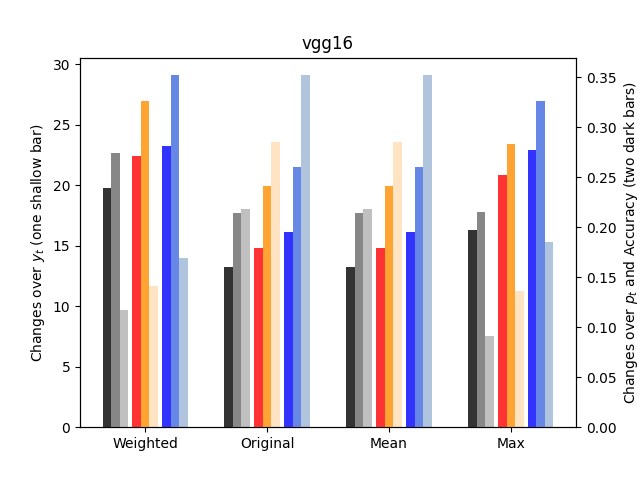
\includegraphics[width = 0.3\textwidth]{figures/grad_sign_perturbation/vgg16_eps003.png} &
    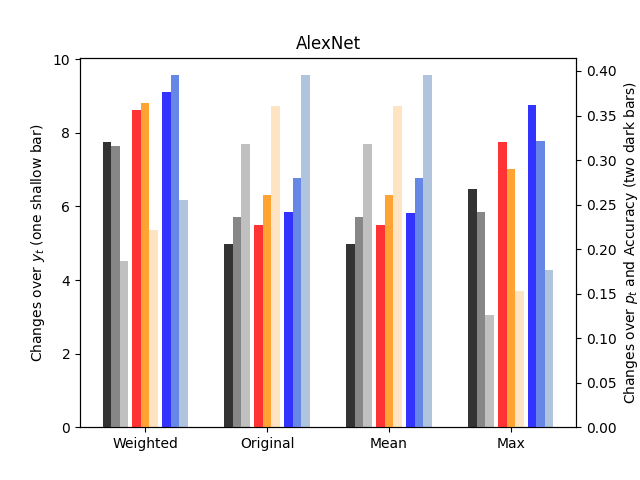
\includegraphics[width = 0.3\textwidth]{figures/grad_sign_perturbation/alexnet_eps003.png} &
    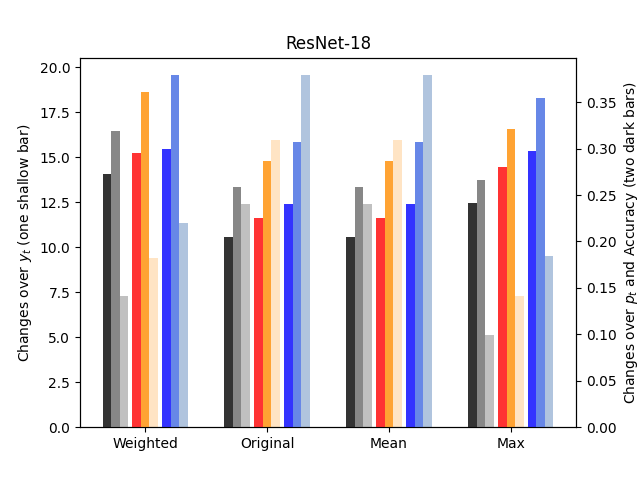
\includegraphics[width = 0.3\textwidth]{figures/grad_sign_perturbation/resnet18_eps003.png} \\

    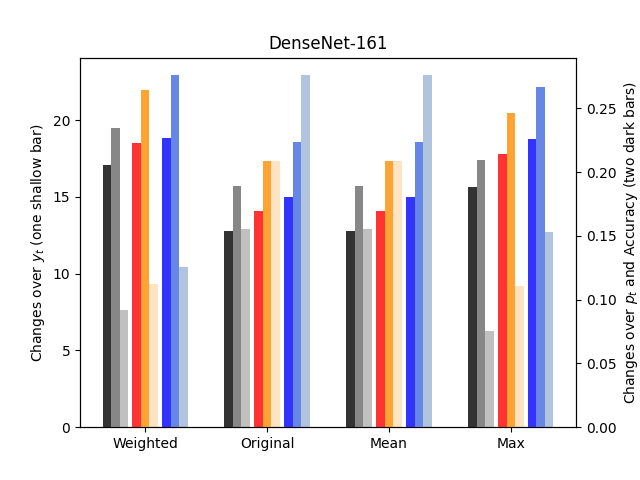
\includegraphics[width = 0.3\textwidth]{figures/grad_sign_perturbation/densenet161_eps003.png} &
    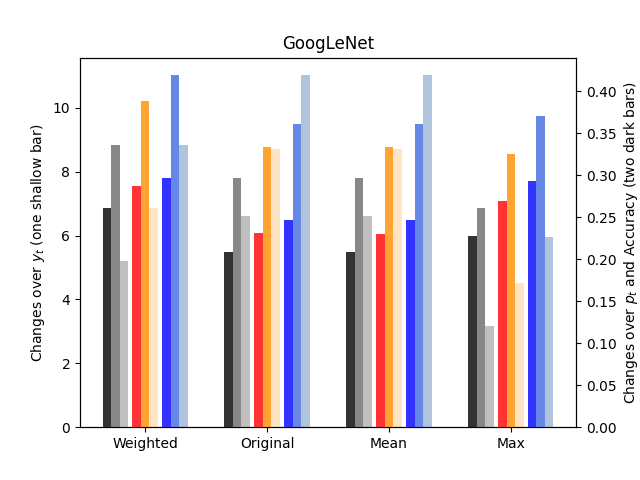
\includegraphics[width = 0.3\textwidth]{figures/grad_sign_perturbation/googlenet_eps003.png} &
    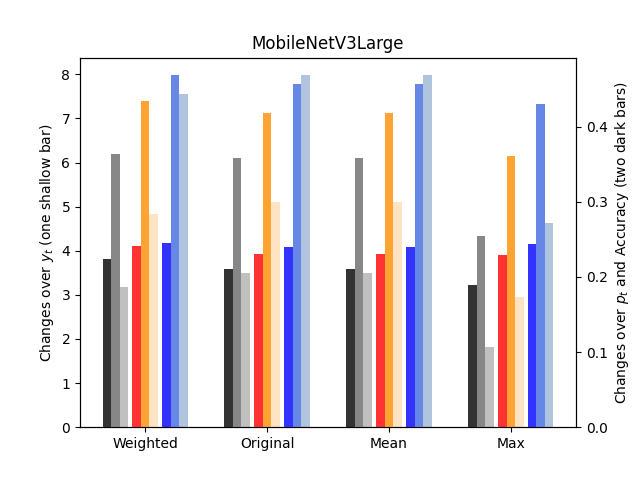
\includegraphics[width = 0.3\textwidth]{figures/grad_sign_perturbation/mobilenetv3large_eps003.png} \\

    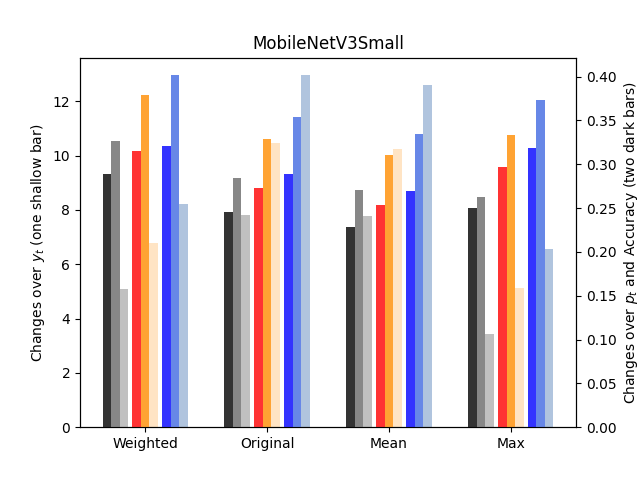
\includegraphics[width = 0.3\textwidth]{figures/grad_sign_perturbation/mobilenetv3small_eps003.png} &
    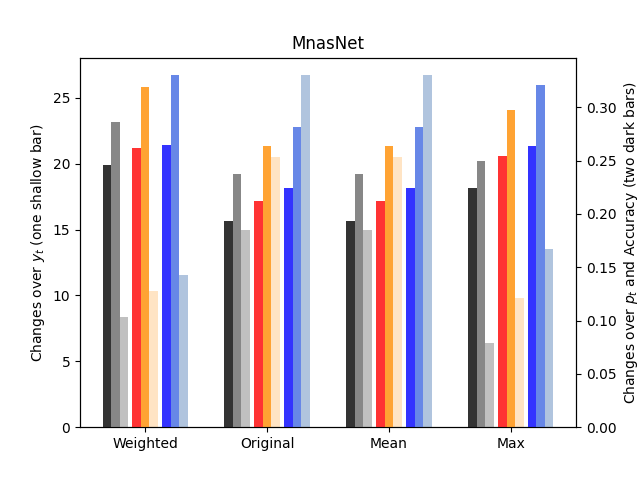
\includegraphics[width = 0.3\textwidth]{figures/grad_sign_perturbation/mnasnet_eps003.png} &
    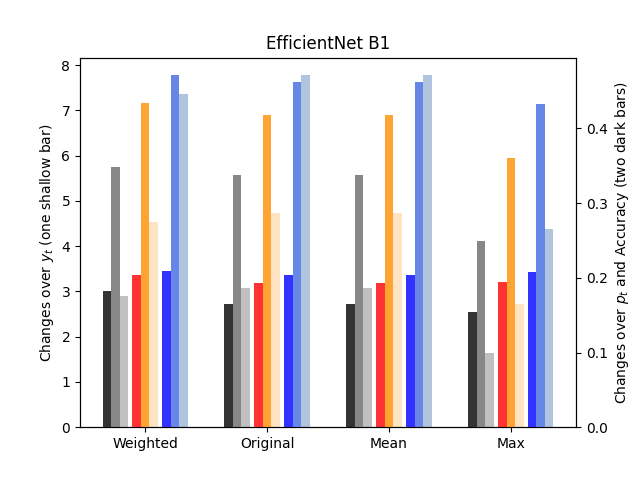
\includegraphics[width = 0.3\textwidth]{figures/grad_sign_perturbation/efficientnetB1_eps003.png} \\

\multicolumn{3}{c}{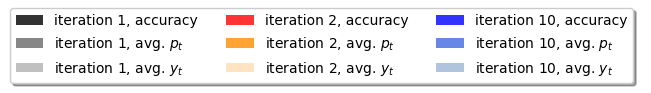
\includegraphics[width = 0.7\textwidth]{figures/grad_sign_perturbation/legend.png} }\\
\end{tabular}
\caption{Reproducing of Figure 3 in the original paper with $\epsilon=\num{3e-3}$. Changes in accuracy, $y_t$ and $p_t$ (t is the target classification class) when certain input features are perturbed. Perturbed features are selected based on four gradient explanations (original, mean, max and weighted), where original is directly with respect to the gradients of the logits.} \label{f:grad_sign_perturbation_eps_003}
\end{figure}


\subsection{Reproducing 5.2 Back-Propagation till the Activation Space}
\label{gradcam_subsection}

This section reproduces section 5.2 in the original paper by performing the same experiments of both visualization and effects of blurring and masking. These experiments were all performed on VGG-16 with batch normalization \citep{vgg16} fine-tuned on the CUB-200 dataset \citep{cub200}. The fine-tuning was done with an SGD optimizer with momentum using a batch size of $128$, learning rate of $10^{-3}$, momentum of $0.9$, and weight decay of $5 \times 10^{-4}$. The model was trained for $200$ epochs on the training set as defined by the dataset. For an exact implementation or to reproduce the model, see our \href{https://anonymous.4open.science/r/contrastive-explanations-58EE/}{repository}. The results of this section generally show evidence for Claim 2, both qualitatively and quantitatively, and show that the proposed weighted contrastive method highlights crucial areas for classification when the model classifies between several dominant classes. The extensions to XGradCAM and FullGrad also show generalizability of the method and thus strengthens Claim 3.

\subsubsection{Visualizations}
Reproduction of the visualizations of three different back-propagation-based methods can be seen in Figure \ref{fig:original_weighted_comp}. Here we compare GradCAM and Linear Approximation, as described in the original paper, and XGradCAM, as described in section \ref{SectionXGradCAM}, to their contrastive weighted counterpart, which was obtained by back-propagating from the softmax neuron $p_t$ of the target class $t$ rather than its logit $y_t$. The visualization was done by overlapping the bilinearly interpolated relevance map on top of the original image with an alpha of $0.5$. A centered norm was applied on the heatmap before visualizing using the \texttt{bwr} colormap in \texttt{Matplotlib}. The images were picked such that $p_2 > 0.1$ and were selected at random to prevent bias from only selecting good samples. Observe that the samples picked are different from those in the original paper as those samples did not have a probability for the second most probable class over the threshold.

The results are partly in line with what the original paper suggests. Firstly, one can note that the original explanation method is quite consistent among the two classes with differences being mostly the intensity of the positive and negative areas. Secondly, one can also see that the weighted methods produce almost complementary heatmaps for the two classes, which makes sense as they are mostly dominant over all other classes. Lastly, we see a large difference in the size of the negative and positive areas visualized compared to the original paper. This is presumably due to different methods of visualization, but as the procedure of visualization of the original paper was not detailed this cannot be confirmed. Observe that the large negative areas in some images, especially seen when comparing our GradCAM to other implementations, are due to the omission of ReLU as described in the original paper. Our results therefore also conflict with the claim in the original paper in appendix G, where the authors claim that non-contrastive methods have much larger positive than negative areas. In Figure \ref{fig:original_weighted_comp} one can see that the original GradCAM has much larger negative areas than positive for all selected images.

\begin{figure}[t]
%\scriptsize
\small
\centering
\resizebox{\textwidth}{!}{\
\begin{tabular}
{ l l c@{\hspace{0.1cm}} c@{\hspace{0.3cm}} c@{\hspace{0.1cm}} c@{\hspace{0.3cm}} c@{\hspace{0.1cm}} c@{\hspace{0.3cm}} c@{\hspace{0.1cm}} c@{\hspace{0.3cm}}}

\toprule
    \multicolumn{2}{l}{\rotatebox[origin=c]{90}{Input}} &
    \multicolumn{2}{c}{$\vcenter{\hbox{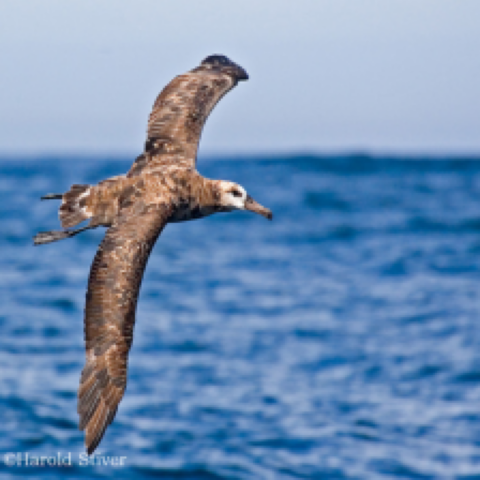
\includegraphics[width = 0.1\textwidth]{figures/Figure 4/2_true_0/input.png}}}$} &
    \multicolumn{2}{c}{$\vcenter{\hbox{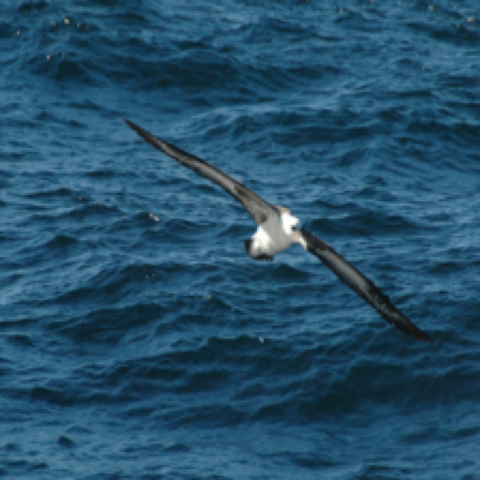
\includegraphics[width = 0.1\textwidth]{figures/Figure 4/51_true_1/input.png}}}$} &
    \multicolumn{2}{c}{$\vcenter{\hbox{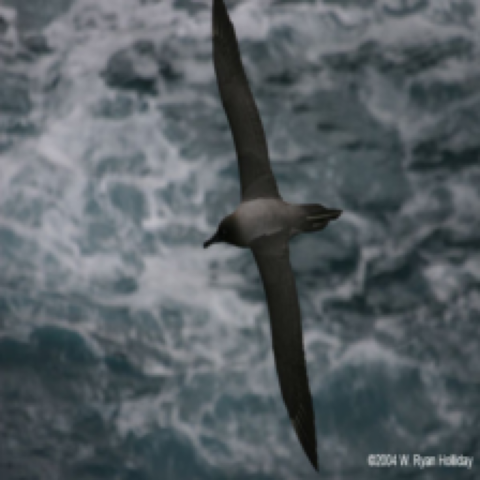
\includegraphics[width = 0.1\textwidth]{figures/Figure 4/85_true_2/input.png}}}$} &
    \multicolumn{2}{c}{$\vcenter{\hbox{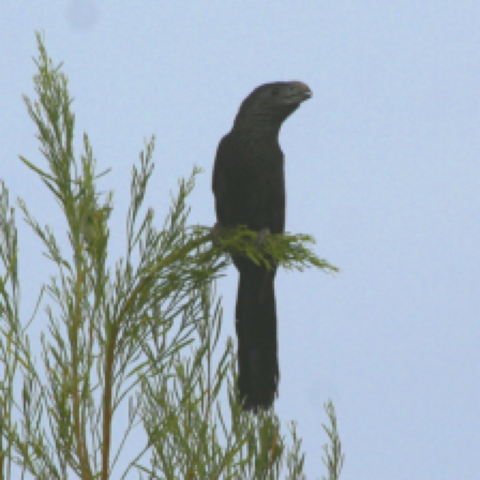
\includegraphics[width = 0.1\textwidth]{figures/Figure 4/116_true_3/input.png}}}$} 
        \vspace{0.1cm}
\\

    &
    &
    $t_1$ &
    $t_2$ &
    $t_1$ &
    $t_2$ &
    $t_1$ &
    $t_2$ &
    $t_1$ &
    $t_2$ \\

\midrule
    \vspace{0.1cm}
    \multirow{2}{*}{\rotatebox[origin=c]{90}{GradCAM }} &
    \rotatebox[origin=c]{90}{Original} &
    $\vcenter{\hbox{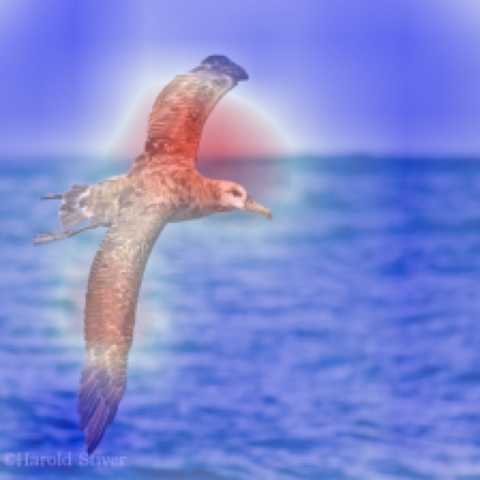
\includegraphics[width = 0.1\textwidth]{figures/Figure 4/2_true_0/gradcam_GC_t1.png}}}$ &
    $\vcenter{\hbox{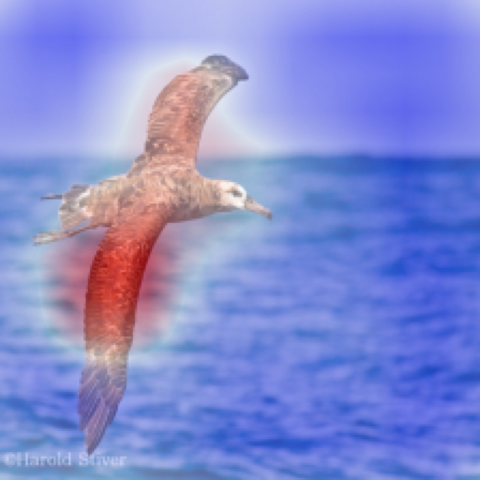
\includegraphics[width = 0.1\textwidth]{figures/Figure 4/2_true_0/gradcam_GC_t2.png}}}$ &
    $\vcenter{\hbox{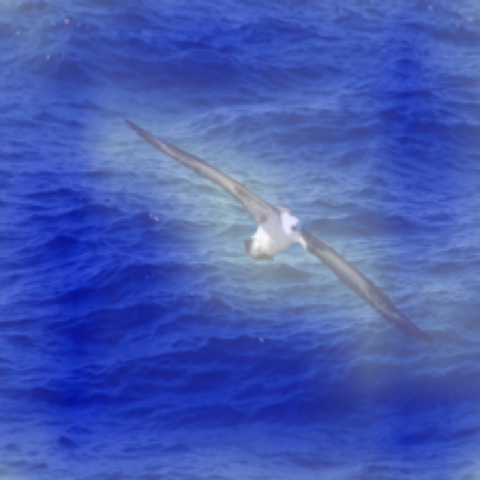
\includegraphics[width = 0.1\textwidth]{figures/Figure 4/51_true_1/gradcam_GC_t1.png}}}$ &
    $\vcenter{\hbox{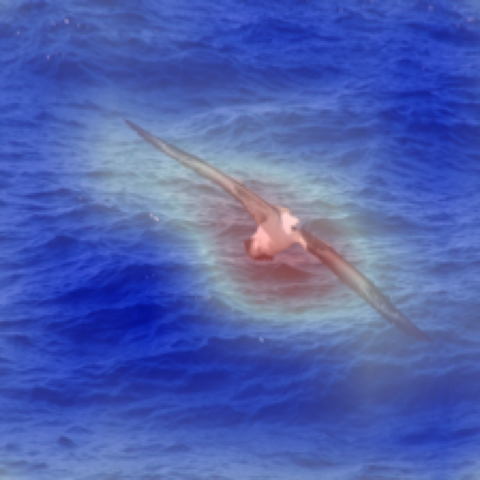
\includegraphics[width = 0.1\textwidth]{figures/Figure 4/51_true_1/gradcam_GC_t2.png}}}$ &
    $\vcenter{\hbox{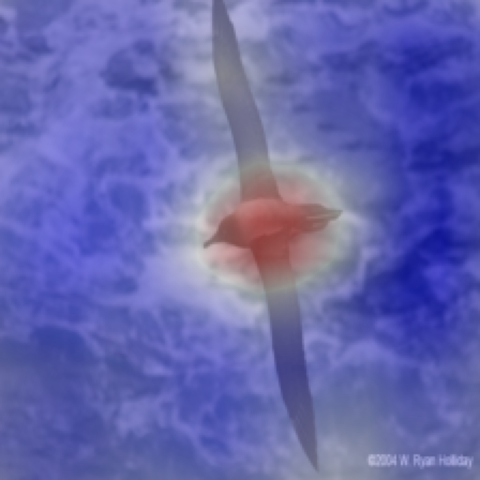
\includegraphics[width = 0.1\textwidth]{figures/Figure 4/85_true_2/gradcam_GC_t1.png}}}$ &
    $\vcenter{\hbox{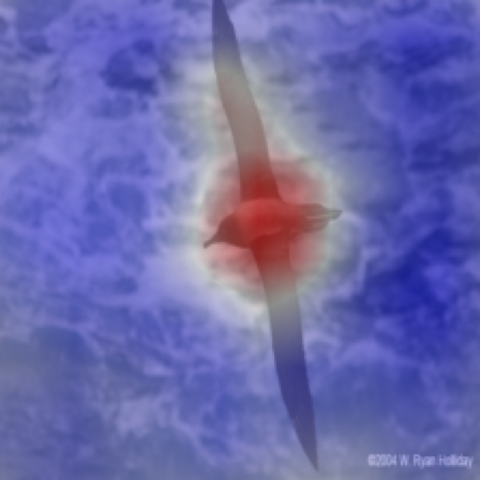
\includegraphics[width = 0.1\textwidth]{figures/Figure 4/85_true_2/gradcam_GC_t2.png}}}$ &
    $\vcenter{\hbox{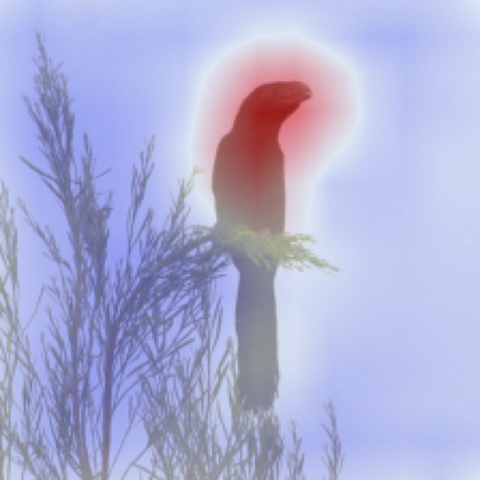
\includegraphics[width = 0.1\textwidth]{figures/Figure 4/116_true_3/gradcam_GC_t1.png}}}$ &
    $\vcenter{\hbox{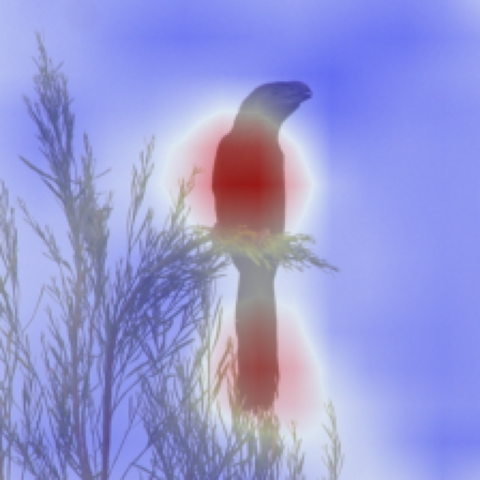
\includegraphics[width = 0.1\textwidth]{figures/Figure 4/116_true_3/gradcam_GC_t2.png}}}$ \\%[1cm]
    
    &
    \rotatebox[origin=c]{90}{Weighted} &
    $\vcenter{\hbox{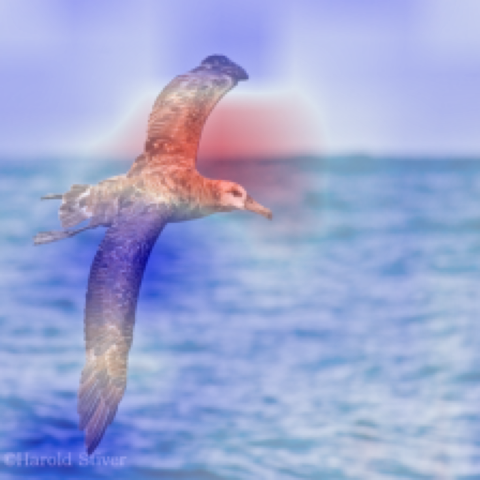
\includegraphics[width = 0.1\textwidth]{figures/Figure 4/2_true_0/contrastive_gradcam_GC_t1.png}}}$ &
    $\vcenter{\hbox{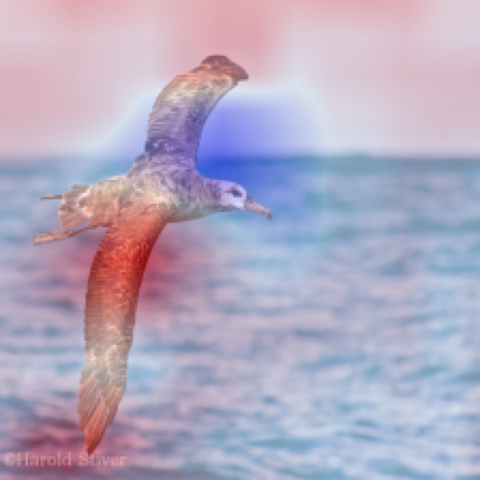
\includegraphics[width = 0.1\textwidth]{figures/Figure 4/2_true_0/contrastive_gradcam_GC_t2.png}}}$ &
    $\vcenter{\hbox{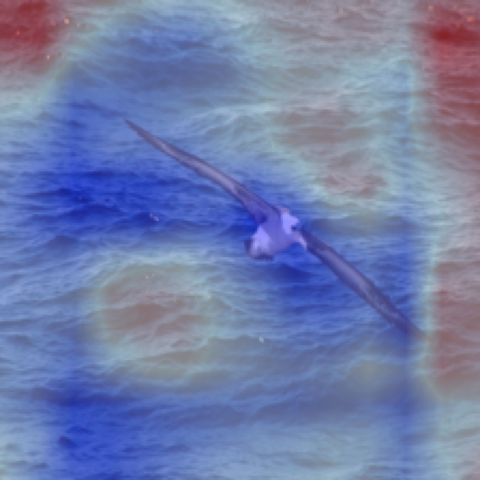
\includegraphics[width = 0.1\textwidth]{figures/Figure 4/51_true_1/contrastive_gradcam_GC_t1.png}}}$ &
    $\vcenter{\hbox{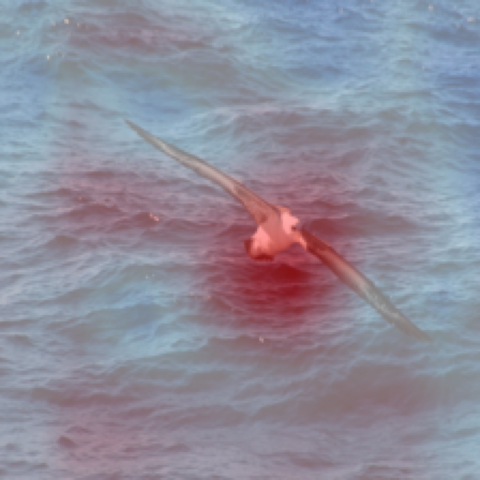
\includegraphics[width = 0.1\textwidth]{figures/Figure 4/51_true_1/contrastive_gradcam_GC_t2.png}}}$ &
    $\vcenter{\hbox{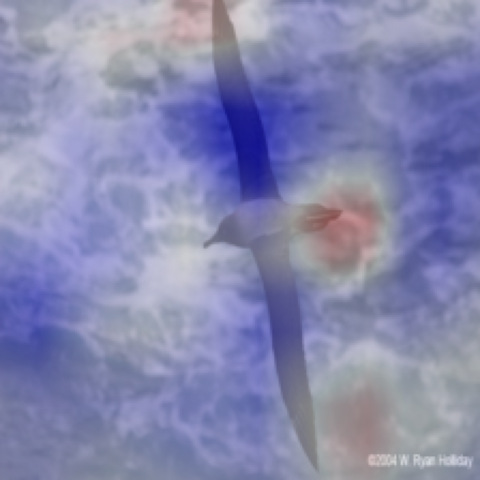
\includegraphics[width = 0.1\textwidth]{figures/Figure 4/85_true_2/contrastive_gradcam_GC_t1.png}}}$ &
    $\vcenter{\hbox{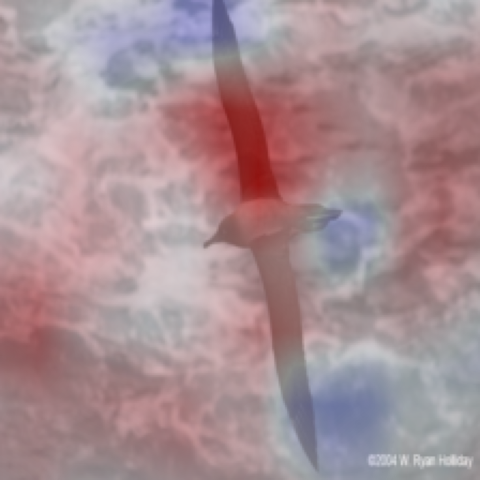
\includegraphics[width = 0.1\textwidth]{figures/Figure 4/85_true_2/contrastive_gradcam_GC_t2.png}}}$ &
    $\vcenter{\hbox{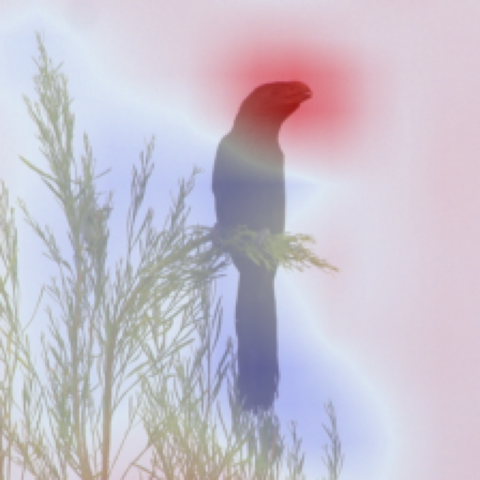
\includegraphics[width = 0.1\textwidth]{figures/Figure 4/116_true_3/contrastive_gradcam_GC_t1.png}}}$ &
    $\vcenter{\hbox{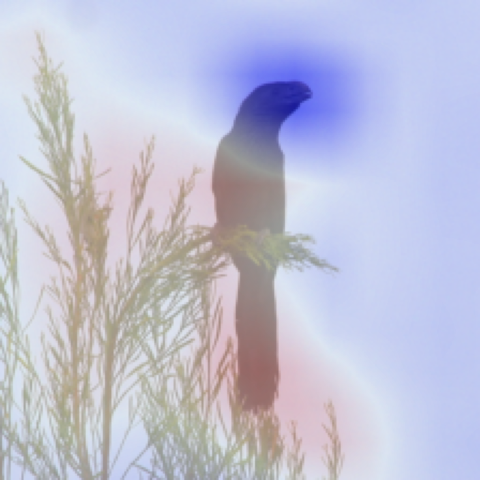
\includegraphics[width = 0.1\textwidth]{figures/Figure 4/116_true_3/contrastive_gradcam_GC_t2.png}}}$ \\

\midrule
    \vspace{0.1cm}
    \multirow{2}{*}{\rotatebox[origin=c]{90}{\shortstack{Linear \\ Approximation}}} &
    \rotatebox[origin=c]{90}{Original} &
    $\vcenter{\hbox{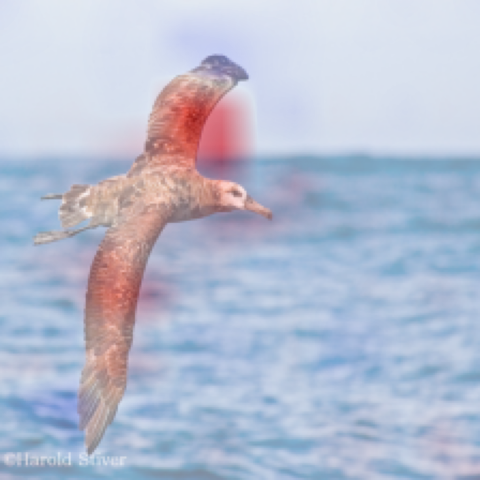
\includegraphics[width = 0.1\textwidth]{figures/Figure 4/2_true_0/gradcam_LA_t1.png}}}$ &
    $\vcenter{\hbox{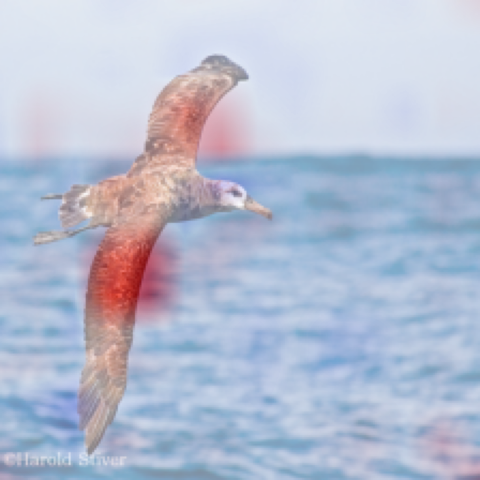
\includegraphics[width = 0.1\textwidth]{figures/Figure 4/2_true_0/gradcam_LA_t2.png}}}$ &
    $\vcenter{\hbox{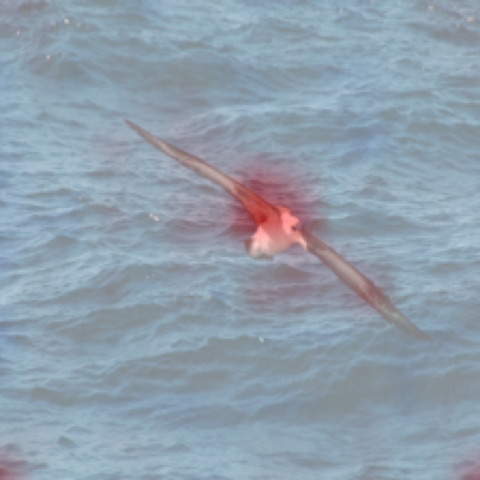
\includegraphics[width = 0.1\textwidth]{figures/Figure 4/51_true_1/gradcam_LA_t1.png}}}$ &
    $\vcenter{\hbox{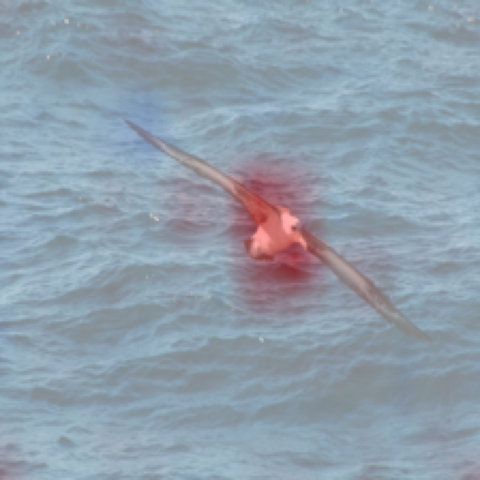
\includegraphics[width = 0.1\textwidth]{figures/Figure 4/51_true_1/gradcam_LA_t2.png}}}$ &
    $\vcenter{\hbox{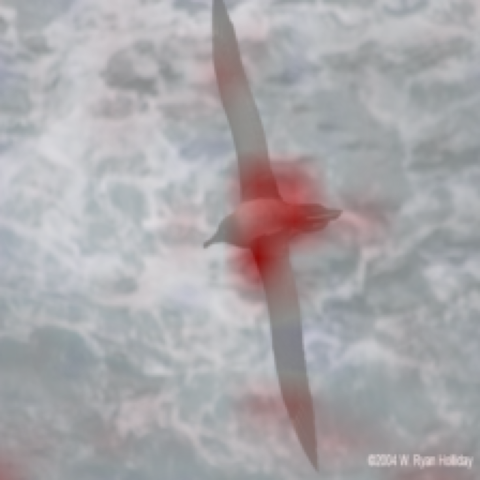
\includegraphics[width = 0.1\textwidth]{figures/Figure 4/85_true_2/gradcam_LA_t1.png}}}$ &
    $\vcenter{\hbox{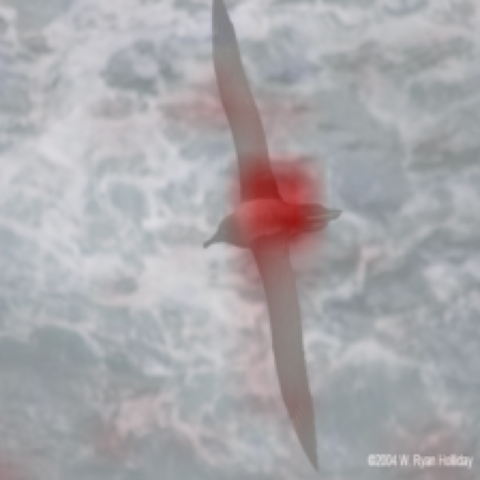
\includegraphics[width = 0.1\textwidth]{figures/Figure 4/85_true_2/gradcam_LA_t2.png}}}$ &
    $\vcenter{\hbox{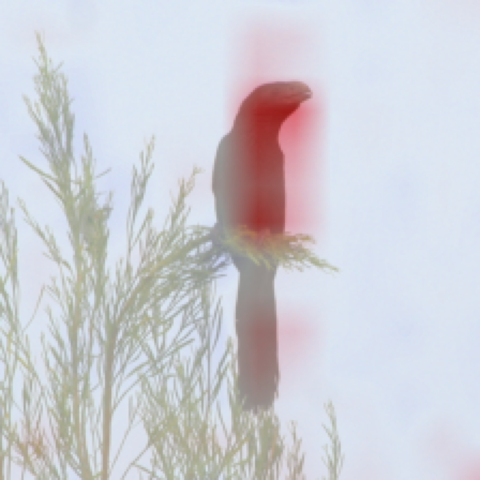
\includegraphics[width = 0.1\textwidth]{figures/Figure 4/116_true_3/gradcam_LA_t1.png}}}$ &
    $\vcenter{\hbox{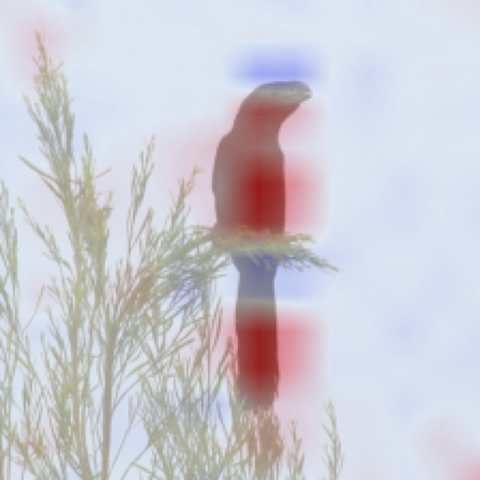
\includegraphics[width = 0.1\textwidth]{figures/Figure 4/116_true_3/gradcam_LA_t2.png}}}$ \\
    
     &
    \rotatebox[origin=c]{90}{Weighted} &
    $\vcenter{\hbox{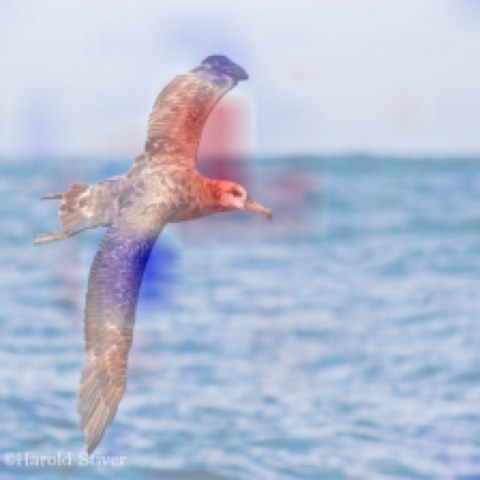
\includegraphics[width = 0.1\textwidth]{figures/Figure 4/2_true_0/contrastive_gradcam_LA_t1.png}}}$ &
    $\vcenter{\hbox{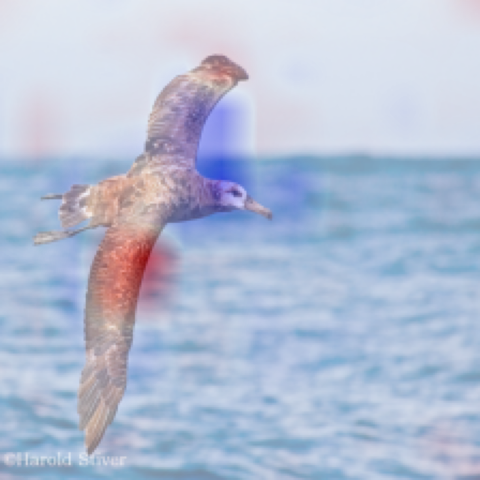
\includegraphics[width = 0.1\textwidth]{figures/Figure 4/2_true_0/contrastive_gradcam_LA_t2.png}}}$ &
    $\vcenter{\hbox{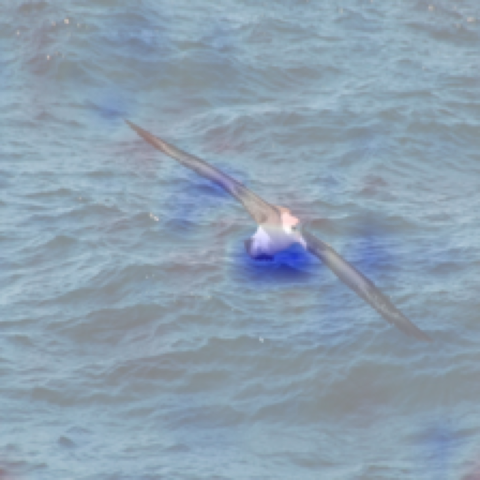
\includegraphics[width = 0.1\textwidth]{figures/Figure 4/51_true_1/contrastive_gradcam_LA_t1.png}}}$ &
    $\vcenter{\hbox{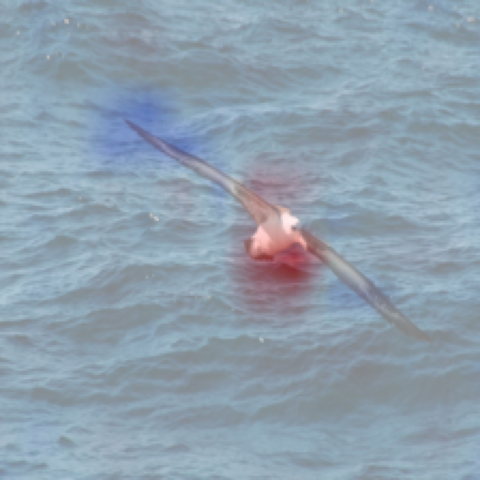
\includegraphics[width = 0.1\textwidth]{figures/Figure 4/51_true_1/contrastive_gradcam_LA_t2.png}}}$ &
    $\vcenter{\hbox{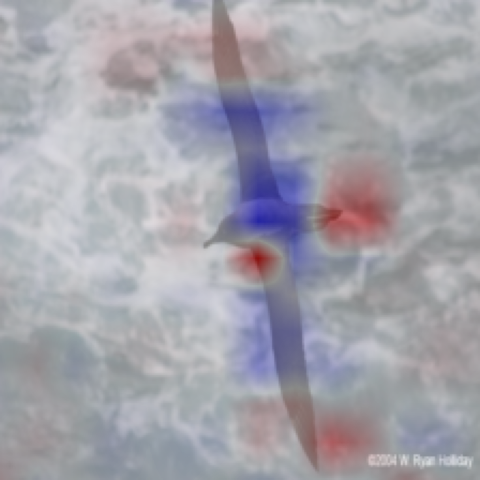
\includegraphics[width = 0.1\textwidth]{figures/Figure 4/85_true_2/contrastive_gradcam_LA_t1.png}}}$ &
    $\vcenter{\hbox{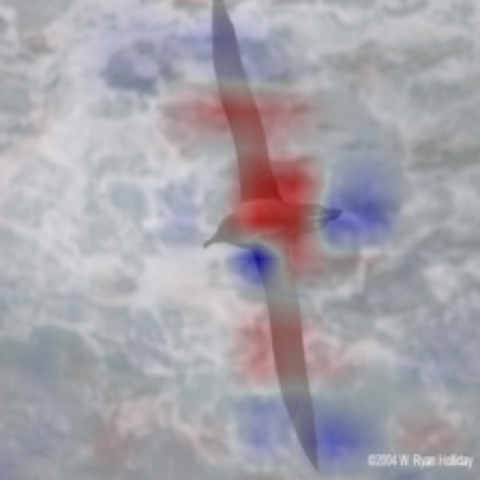
\includegraphics[width = 0.1\textwidth]{figures/Figure 4/85_true_2/contrastive_gradcam_LA_t2.png}}}$ &
    $\vcenter{\hbox{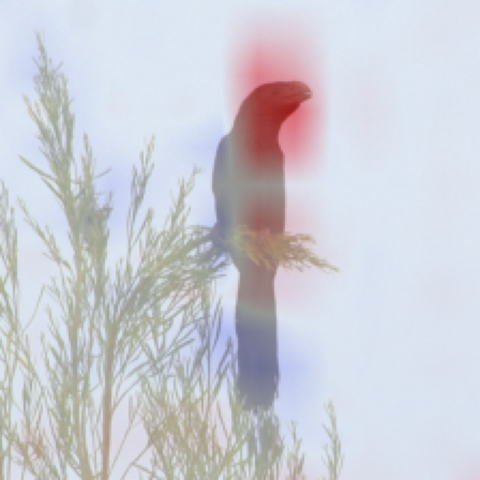
\includegraphics[width = 0.1\textwidth]{figures/Figure 4/116_true_3/contrastive_gradcam_LA_t1.png}}}$ &
    $\vcenter{\hbox{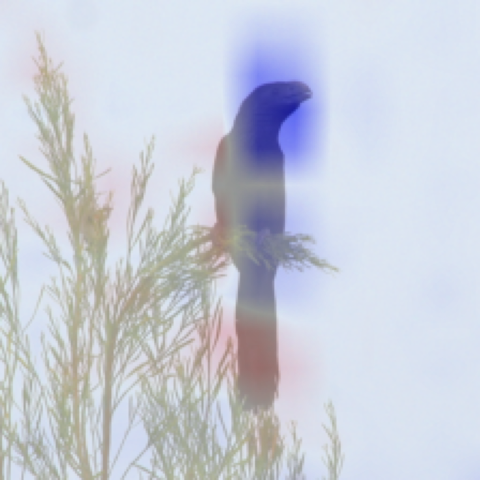
\includegraphics[width = 0.1\textwidth]{figures/Figure 4/116_true_3/contrastive_gradcam_LA_t2.png}}}$ \\

\midrule
    \vspace{0.1cm}
    \multirow{2}{*}{\rotatebox[origin=c]{90}{\shortstack{XGradCAM }}} &
    \rotatebox[origin=c]{90}{Original} &
    $\vcenter{\hbox{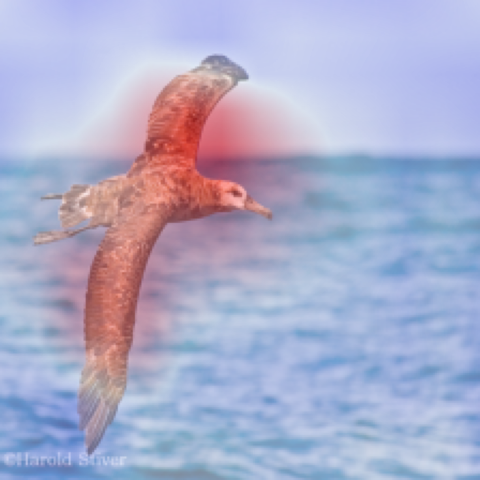
\includegraphics[width = 0.1\textwidth]{figures/Figure 4/2_true_0/gradcam_XC_t1.png}}}$ &
    $\vcenter{\hbox{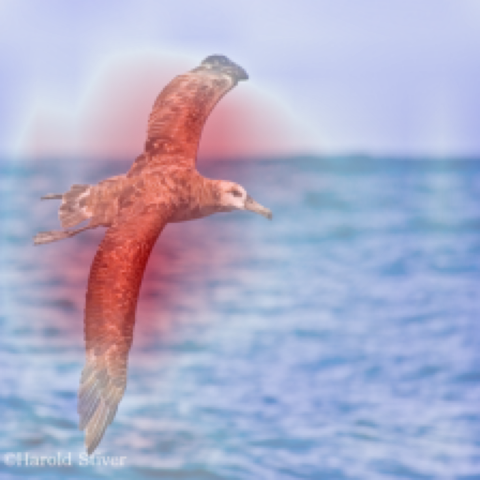
\includegraphics[width = 0.1\textwidth]{figures/Figure 4/2_true_0/gradcam_XC_t2.png}}}$ &
    $\vcenter{\hbox{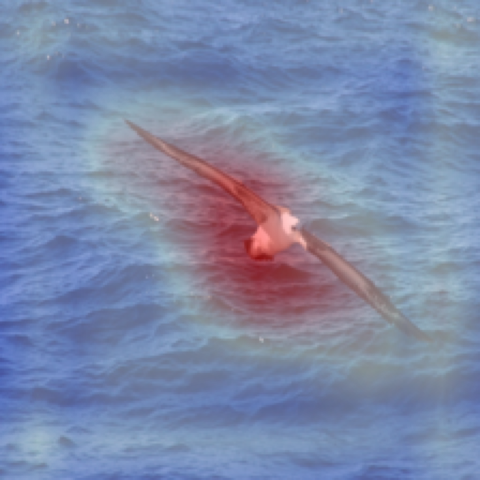
\includegraphics[width = 0.1\textwidth]{figures/Figure 4/51_true_1/gradcam_XC_t1.png}}}$ &
    $\vcenter{\hbox{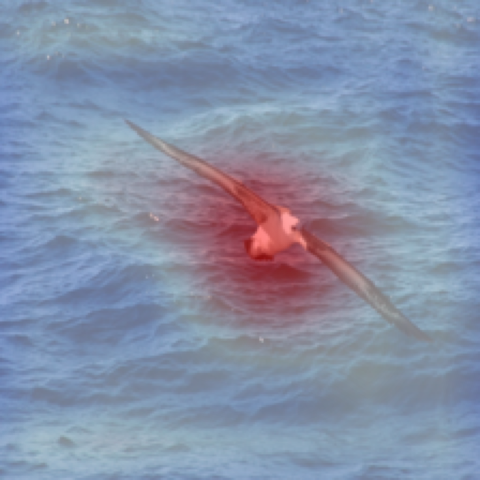
\includegraphics[width = 0.1\textwidth]{figures/Figure 4/51_true_1/gradcam_XC_t2.png}}}$ &
    $\vcenter{\hbox{\includegraphics[width = 0.1\textwidth]{figures/Figure 4/85_true_2/gradcam_XC_t1.png}}}$ &
    $\vcenter{\hbox{\includegraphics[width = 0.1\textwidth]{figures/Figure 4/85_true_2/gradcam_XC_t2.png}}}$ &
    $\vcenter{\hbox{\includegraphics[width = 0.1\textwidth]{figures/Figure 4/116_true_3/gradcam_XC_t1.png}}}$ &
    $\vcenter{\hbox{\includegraphics[width = 0.1\textwidth]{figures/Figure 4/116_true_3/gradcam_XC_t2.png}}}$ \\
    
     &
    \rotatebox[origin=c]{90}{Weighted} &
    $\vcenter{\hbox{\includegraphics[width = 0.1\textwidth]{figures/Figure 4/2_true_0/contrastive_gradcam_XC_t1.png}}}$ &
    $\vcenter{\hbox{\includegraphics[width = 0.1\textwidth]{figures/Figure 4/2_true_0/contrastive_gradcam_XC_t2.png}}}$ &
    $\vcenter{\hbox{\includegraphics[width = 0.1\textwidth]{figures/Figure 4/51_true_1/contrastive_gradcam_XC_t1.png}}}$ &
    $\vcenter{\hbox{\includegraphics[width = 0.1\textwidth]{figures/Figure 4/51_true_1/contrastive_gradcam_XC_t2.png}}}$ &
    $\vcenter{\hbox{\includegraphics[width = 0.1\textwidth]{figures/Figure 4/85_true_2/contrastive_gradcam_XC_t1.png}}}$ &
    $\vcenter{\hbox{\includegraphics[width = 0.1\textwidth]{figures/Figure 4/85_true_2/contrastive_gradcam_XC_t2.png}}}$ &
    $\vcenter{\hbox{\includegraphics[width = 0.1\textwidth]{figures/Figure 4/116_true_3/contrastive_gradcam_XC_t1.png}}}$ &
    $\vcenter{\hbox{\includegraphics[width = 0.1\textwidth]{figures/Figure 4/116_true_3/contrastive_gradcam_XC_t2.png}}}$ \\
\bottomrule
\end{tabular} }
\caption{Reproduction of Figure 4 in the original paper. Comparison between the back-propagation from logits $y_t$ (Original) and weighted contrastive
back-propagation from $p_t$ (Weighted) for GradCAM, Linear Approximation, and XGradCAM. The columns for each image signify the most possible and second possible class, respectively. Red and blue signal positive and negative activations respectively.} \label{fig:original_weighted_comp}
\end{figure}

The same experiments when performed using FullGrad produce fully negative saliency maps. The modified FullGrad is therefore not truly contrastive as it does not have both positive and negative contributions instead one has to use normalization and assume that they are evenly distributed. When normalizing is applied to the final saliency map the results are similar to those seen in Figure \ref{fig:original_weighted_comp} and some select images can be seen in Figure \ref{fig:fullgrad}. These seem to be of a more fine-grained nature than the GradCAM-based methods in Figure \ref{fig:original_weighted_comp} while largely highlighting the same areas. This suggests a suitable alternative to GradCAM-based methods and that a contrastive visualization is possible for FullGrad but that this relies on normalization.

\begin{figure}[t]
%\scriptsize
\small
\centering
\resizebox{0.8\textwidth}{!}{\
\begin{tabular}
{ l l c@{\hspace{0.1cm}} c@{\hspace{0.3cm}} c@{\hspace{0.1cm}} c@{\hspace{0.3cm}} c@{\hspace{0.1cm}} c@{\hspace{0.3cm}} c@{\hspace{0.1cm}} c@{\hspace{0.3cm}}}

\toprule
    \multicolumn{2}{l}{\rotatebox[origin=c]{90}{Input}} &
    \multicolumn{2}{c}{$\vcenter{\hbox{\includegraphics[width = 0.1\textwidth]{figures/Figure 4/2_true_0/input.png}}}$} &
    \multicolumn{2}{c}{$\vcenter{\hbox{\includegraphics[width = 0.1\textwidth]{figures/Figure 4/51_true_1/input.png}}}$} &
    \multicolumn{2}{c}{$\vcenter{\hbox{\includegraphics[width = 0.1\textwidth]{figures/Figure 4/85_true_2/input.png}}}$} &
        \vspace{0.1cm}
\\

    &
    &
    $t_1$ &
    $t_2$ &
    $t_1$ &
    $t_2$ &
    $t_1$ &
    $t_2$ &\\

\midrule
    \vspace{0.1cm}
    \multirow{2}{*}{\rotatebox[origin=c]{90}{FullGrad}} &
    \rotatebox[origin=c]{90}{Original} &
    $\vcenter{\hbox{\includegraphics[width = 0.1\textwidth]{figures/Figure 4/2_true_0/gradcam_FG_t1.png}}}$ &
    $\vcenter{\hbox{\includegraphics[width = 0.1\textwidth]{figures/Figure 4/2_true_0/gradcam_FG_t2.png}}}$ &
    $\vcenter{\hbox{\includegraphics[width = 0.1\textwidth]{figures/Figure 4/51_true_1/gradcam_FG_t1.png}}}$ &
    $\vcenter{\hbox{\includegraphics[width = 0.1\textwidth]{figures/Figure 4/51_true_1/gradcam_FG_t2.png}}}$ &
    $\vcenter{\hbox{\includegraphics[width = 0.1\textwidth]{figures/Figure 4/85_true_2/gradcam_FG_t1.png}}}$ &
    $\vcenter{\hbox{\includegraphics[width = 0.1\textwidth]{figures/Figure 4/85_true_2/gradcam_FG_t2.png}}}$ \\%[1cm]
    
    &
    \rotatebox[origin=c]{90}{Weighted} &
    $\vcenter{\hbox{\includegraphics[width = 0.1\textwidth]{figures/Figure 4/2_true_0/contrastive_gradcam_FG_t1.png}}}$ &
    $\vcenter{\hbox{\includegraphics[width = 0.1\textwidth]{figures/Figure 4/2_true_0/contrastive_gradcam_FG_t2.png}}}$ &
    $\vcenter{\hbox{\includegraphics[width = 0.1\textwidth]{figures/Figure 4/51_true_1/contrastive_gradcam_FG_t1.png}}}$ &
    $\vcenter{\hbox{\includegraphics[width = 0.1\textwidth]{figures/Figure 4/51_true_1/contrastive_gradcam_FG_t2.png}}}$ &
    $\vcenter{\hbox{\includegraphics[width = 0.1\textwidth]{figures/Figure 4/85_true_2/contrastive_gradcam_FG_t1.png}}}$ &
    $\vcenter{\hbox{\includegraphics[width = 0.1\textwidth]{figures/Figure 4/85_true_2/contrastive_gradcam_FG_t2.png}}}$ \\

\bottomrule
\end{tabular} }
\caption{Comparison between the back-propagation from logits $y_t$ (Original) and weighted contrastive
back-propagation from $p_t$ (Weighted) for FullGrad. The columns for each image signify the most possible and second possible class, respectively. Red and blue signal positive and negative activations respectively after normalization.} \label{fig:fullgrad}
\end{figure}

\subsubsection{Blurring and masking}
Reproduction of the blurring and masking experiment seen in Table 1 of the original paper can be seen in Table \ref{t:blurring}. Here we also added an additional row with results using XGradCAM. FullGrad is not analyzed as the modified version only produces negative areas. This gave similar results to GradCAM and Linear Approximation although performed slightly better on the negative features and for positive features for the second most probable class $t_2$. Here we use the same baselines as the original paper with the motivation of them having slightly different results without a generally accepted standard \citep{baselinesimpact}. The values in the table are the average relative probability of the most and second most probable classes for each image. This relative probability is defined as $\Bar{p}_{t_i} = \mathbb{E}\left[e^{y_{t_i}} / (e^{y_{t_1}} + e^{y_{t_2}})  \right], i=1,2$ where $t_i \in [c]$ represents the $i$-th most possible class. These expectations are, like in the original paper, only calculated over samples that fulfill the threshold criteria $p_2 > 0.1$.

The results are very similar to those of the original paper, although not identical, and show the same patterns. We decided to use equal blurring and masking here to prevent bias where one method might yield larger or smaller negative areas to guarantee that the original and weighted methods both modify an equal number of pixels. This was also suggested in the original paper in appendix G and seems to have a minor impact on the results while negating some bias.
% We want to emphasize, however, that these results are expected since the weighted method back-propagates from the softmax neuron $p_t$, and therefore blurring using that method will impact the resulting activation of the very same neuron more than back-propagating from the preceding logit $y_t$. 

\begin{table}
    \tiny
    
    %\fontfamily{lmodern}\selectfont % Set font family to Latin Modern Sans Serif
    
    \centering
    \caption{Reproduction of Table 1 in the original paper using equal blurring. Comparisons between weighted contrastive method (wtd.) and original method (ori.) when blurring and masking. Using baselines Gaussian Blur, Zeros, and Channel-wise Mean and the methods Linear Approximation (LA), GradCAM (GC), and XGradCAM (XC). $t_1$ and $t_2$ are the classes with the highest and second highest probability respectively. Each line shows how the average relative probability changes among each image's top two classes. Pos. and Neg. Features mean that only positive and negative features are kept with respect to the corresponding target class. It is expected that when the positive or negative features corresponding to the target are kept, the expected relative probability is expected to increase or decrease respectively.} \label{t:blurring}
    \vspace{2mm}
    \resizebox{\textwidth}{!}{\
    \begin{tabular}{c | c | c | c | c  c | c  c | c  c | c  c | c  c | c  c}
    %\abovetopsep
    \toprule
    %\hline
        \multicolumn{3}{c |}{} &
        \multirow{3}{*}{$p_t$} &
        \multicolumn{4}{c |}{Gaussian Blur} &
        \multicolumn{4}{c |}{Zeros} &
        \multicolumn{4}{c}{Channel-wise Mean} \\ \cline{5-16}

        \multicolumn{3}{c |}{} &
        &
        \multicolumn{2}{c |}{Pos. Features} &
        \multicolumn{2}{c |}{Neg. Features} &
        \multicolumn{2}{c |}{Pos. Features} &
        \multicolumn{2}{c |}{Neg. Features} &
        \multicolumn{2}{c |}{Pos. Features} &
        \multicolumn{2}{c}{Neg. Features} \\ \cline{5-16}

        \multicolumn{3}{c |}{} &
        &
        ori. &
        wtd. &
        ori. &
        wtd. &
        ori. &
        wtd. &
        ori. &
        wtd. &
        ori. &
        wtd. &
        ori. &
        wtd.\\

        \midrule

        \multirow{6}{*}{CUB-200} &
        \multirow{2}{*}{LA} &
        $t_1$ &
        0.712 &
        0.695 &
        \textbf{0.789} &
        0.419 &
        \textbf{0.274} &
        0.663 &
        \textbf{0.754} &
        0.428 &
        \textbf{0.292} &
        0.676 &
        \textbf{0.766} &
        0.426 &
        \textbf{0.281} \\

         &
         &
        $t_2$ &
        0.288 &
        0.560 &
        \textbf{0.738} &
        0.390 &
        \textbf{0.211} &
        0.563 &
        \textbf{0.717} &
        0.398 &
        \textbf{0.253} &
        0.558 &
        \textbf{0.729} &
        0.391 &
        \textbf{0.235} \\

         &
        \multirow{2}{*}{GC} &
        $t_1$ &
        0.712 &
        0.747 &
        \textbf{0.858} &
        0.428 &
        \textbf{0.271} &
        0.731 &
        \textbf{0.850} &
        0.432 &
        \textbf{0.286} &
        0.745 &
        \textbf{0.857} &
        0.426 &
        \textbf{0.277} \\

         &
         &
        $t_2$ &
        0.288 &
        0.461 &
        \textbf{0.759} &
        0.402 &
        \textbf{0.199} &
        0.469 &
        \textbf{0.761} &
        0.414 &
        \textbf{0.226} &
        0.468 &
        \textbf{0.759} &
        0.406 &
        \textbf{0.214} \\

         &
        \multirow{2}{*}{XC} &
        $t_1$ &
        0.712 &
        0.733 &
        \textbf{0.847} &
        0.422 &
        \textbf{0.248} &
        0.711 &
        \textbf{0.838} &
        0.426 &
        \textbf{0.266} &
        0.719 &
        \textbf{0.844} &
        0.419 &
        \textbf{0.253} \\

         &
         &
        $t_2$ &
        0.288 &
        0.504 &
        \textbf{0.785} &
        0.393 &
        \textbf{0.169} &
        0.515 &
        \textbf{0.777} &
        0.402 &
        \textbf{0.184} &
        0.511 &
        \textbf{0.784} &
        0.395 &
        \textbf{0.177} \\
    \midrule
    \end{tabular} }
\end{table}



\subsection{Reproducing 5.3 Comparison with Mean/Max Contrast}

We perform the same experiments as in section 5.3 of the original article. Here we reuse the same VGG-16 model used in section \ref{gradcam_subsection} and implement mean and max contrast as described in the original paper. The used method for visualization is also the same as in section \ref{gradcam_subsection} and a threshold of $p_3 > 0.1$ is used. The results, seen in Figure \ref{f:meanmaxcomp}, are similar to the original paper, especially the observation that original and mean methods yield extremely similar results due to the tiny scaling factor used when subtracting by the other classes in the mean method. We also note that max similarity for the two most probable classes is each other's inverse and that the weighted method gives a similar but more detailed comparison that includes several classes simultaneously. Like in section \ref{gradcam_subsection} we also observe that the negative areas are much larger than in the compared article, presumably due to different visualization methods.

Figure \ref{f:meanmaxcomp} also highlights the strengths of the weighted contrastive method. Here it is clear that the weighted method helps give detail to which areas of the image are key for a specific classification given a choice of several dominating classes. This can be useful when debugging misclassified samples where positive regions using the weighted method indicate regions that the model considered in its choice. For example, for the top-left part of Figure \ref{f:meanmaxcomp} one can clearly see that the top class puts a heavy bias on a few select spots of the background, thus indicating that the model might be utilizing non-object pixels to classify the object. This is further evidence for Claim 2.
\begin{figure}[t]
\tiny

%\fontfamily{lmss}\selectfont % Set font family to Latin Modern Sans Serif

\centering
\begin{tabular}
{ 
c@{\hspace{0.09cm}} c@{\hspace{0.09cm}} c@{\hspace{0.09cm}} c@{\hspace{0.09cm}} c@{\hspace{0.09cm}} c@{\hspace{0.09cm}} c@{\hspace{0.09cm}} c@{\hspace{0.09cm}} c@{\hspace{0.09cm}} c@{\hspace{0.09cm}}}
\toprule
    &
    \multicolumn{4}{c}{$\vcenter{\hbox{\textbf{Laysan albatross}}}$} &
    &
    \multicolumn{4}{c}{$\vcenter{\hbox{\textbf{Laysan albatross}}}$} \\
    
    &
    \multicolumn{4}{c}{ $\vcenter{\hbox{\includegraphics[width = 0.08\textwidth]{figures/Figure 5/42_true_1/input.png}}}$ } &
    &
    \multicolumn{4}{c}{$\vcenter{\hbox{\includegraphics[width = 0.08\textwidth]{figures/Figure 5/34_true_1/input.png}}}$} \\

    &
    original &
    mean &
    max &
    weighted &
    &
    original &
    mean &
    max &
    weighted \\
    
    \vspace{0.09cm}
    $\vcenter{\hbox{\shortstack{Explanation for: \\ \textbf{Long-tailed jaeger} \\p=0.451}}}$ &
    $\vcenter{\hbox{\includegraphics[width = 0.08\textwidth]{figures/Figure 5/42_true_1/original_GC_t1_70_0.451.png}}}$ &
    $\vcenter{\hbox{\includegraphics[width = 0.08\textwidth]{figures/Figure 5/42_true_1/mean_GC_t1_70_0.451.png}}}$ &
    $\vcenter{\hbox{\includegraphics[width = 0.08\textwidth]{figures/Figure 5/42_true_1/max_GC_t1_70_0.451.png}}}$ &
    $\vcenter{\hbox{\includegraphics[width = 0.08\textwidth]{figures/Figure 5/42_true_1/weighted_GC_t1_70_0.451.png}}}$ &
    $\vcenter{\hbox{\shortstack{Explanation for: \\ \textbf{Sooty albatross} \\p=0.354}}}$ &
    $\vcenter{\hbox{\includegraphics[width = 0.08\textwidth]{figures/Figure 5/34_true_1/original_GC_t1_2_0.354.png}}}$ &
    $\vcenter{\hbox{\includegraphics[width = 0.08\textwidth]{figures/Figure 5/34_true_1/mean_GC_t1_2_0.354.png}}}$ &
    $\vcenter{\hbox{\includegraphics[width = 0.08\textwidth]{figures/Figure 5/34_true_1/max_GC_t1_2_0.354.png}}}$ &
    $\vcenter{\hbox{\includegraphics[width = 0.08\textwidth]{figures/Figure 5/34_true_1/weighted_GC_t1_2_0.354.png}}}$ \\

    \vspace{0.09cm}
    $\vcenter{\hbox{\shortstack{Explanation for: \\ \textbf{Laysan albatross} \\p=0.279}}}$ &
    $\vcenter{\hbox{\includegraphics[width = 0.08\textwidth]{figures/Figure 5/42_true_1/original_GC_t2_1_0.279.png}}}$ &
    $\vcenter{\hbox{\includegraphics[width = 0.08\textwidth]{figures/Figure 5/42_true_1/mean_GC_t2_1_0.279.png}}}$ &
    $\vcenter{\hbox{\includegraphics[width = 0.08\textwidth]{figures/Figure 5/42_true_1/max_GC_t2_1_0.279.png}}}$ &
    $\vcenter{\hbox{\includegraphics[width = 0.08\textwidth]{figures/Figure 5/42_true_1/weighted_GC_t2_1_0.279.png}}}$ &
    $\vcenter{\hbox{\shortstack{Explanation for: \\ \textbf{White pelican} \\p=0.214}}}$ &
    $\vcenter{\hbox{\includegraphics[width = 0.08\textwidth]{figures/Figure 5/34_true_1/original_GC_t2_100_0.214.png}}}$ &
    $\vcenter{\hbox{\includegraphics[width = 0.08\textwidth]{figures/Figure 5/34_true_1/mean_GC_t2_100_0.214.png}}}$ &
    $\vcenter{\hbox{\includegraphics[width = 0.08\textwidth]{figures/Figure 5/34_true_1/max_GC_t2_100_0.214.png}}}$ &
    $\vcenter{\hbox{\includegraphics[width = 0.08\textwidth]{figures/Figure 5/34_true_1/weighted_GC_t2_100_0.214.png}}}$ \\
    \vspace{0.09cm}
    $\vcenter{\hbox{\shortstack{Explanation for: \\ \textbf{Geococcyx} \\p=0.134}}}$ &
    $\vcenter{\hbox{\includegraphics[width = 0.08\textwidth]{figures/Figure 5/42_true_1/original_GC_t3_109_0.134.png}}}$ &
    $\vcenter{\hbox{\includegraphics[width = 0.08\textwidth]{figures/Figure 5/42_true_1/mean_GC_t3_109_0.134.png}}}$ &
    $\vcenter{\hbox{\includegraphics[width = 0.08\textwidth]{figures/Figure 5/42_true_1/max_GC_t3_109_0.134.png}}}$ &
    $\vcenter{\hbox{\includegraphics[width = 0.08\textwidth]{figures/Figure 5/42_true_1/weighted_GC_t3_109_0.134.png}}}$ &
    $\vcenter{\hbox{\shortstack{Explanation for: \\ \textbf{Frigatebird} \\p=0.194}}}$ &
    $\vcenter{\hbox{\includegraphics[width = 0.08\textwidth]{figures/Figure 5/34_true_1/original_GC_t3_43_0.194.png}}}$ &
    $\vcenter{\hbox{\includegraphics[width = 0.08\textwidth]{figures/Figure 5/34_true_1/mean_GC_t3_43_0.194.png}}}$ &
    $\vcenter{\hbox{\includegraphics[width = 0.08\textwidth]{figures/Figure 5/34_true_1/max_GC_t3_43_0.194.png}}}$ &
    $\vcenter{\hbox{\includegraphics[width = 0.08\textwidth]{figures/Figure 5/34_true_1/weighted_GC_t3_43_0.194.png}}}$ \\

\midrule
    &
    \multicolumn{4}{c}{$\vcenter{\hbox{\textbf{Brewer blackbird}}}$} &
    &
    \multicolumn{4}{c}{$\vcenter{\hbox{\textbf{Eastern towhee}}}$} \\
    
    &
    \multicolumn{4}{c}{$\vcenter{\hbox{\includegraphics[width = 0.08\textwidth]{figures/Figure 5/194_true_8/input.png}}}$} &
    &
    \multicolumn{4}{c}{$\vcenter{\hbox{\includegraphics[width = 0.08\textwidth]{figures/Figure 5/542_true_20/input.png}}}$} \\

    &
    original &
    mean &
    max &
    weighted &
    &
    original &
    mean &
    max &
    weighted \\
    
    \vspace{0.09cm}
    $\vcenter{\hbox{\shortstack{Explanation for: \\ \textbf{American crow} \\p=0.334}}}$ &
    $\vcenter{\hbox{\includegraphics[width = 0.08\textwidth]{figures/Figure 5/194_true_8/original_GC_t1_28_0.334.png}}}$ &
    $\vcenter{\hbox{\includegraphics[width = 0.08\textwidth]{figures/Figure 5/194_true_8/mean_GC_t1_28_0.334.png}}}$ &
    $\vcenter{\hbox{\includegraphics[width = 0.08\textwidth]{figures/Figure 5/194_true_8/max_GC_t1_28_0.334.png}}}$ &
    $\vcenter{\hbox{\includegraphics[width = 0.08\textwidth]{figures/Figure 5/194_true_8/weighted_GC_t1_28_0.334.png}}}$ &
    $\vcenter{\hbox{\shortstack{Explanation for: \\ \textbf{Orchard oriole} \\p=0.573}}}$ &
    $\vcenter{\hbox{\includegraphics[width = 0.08\textwidth]{figures/Figure 5/542_true_20/original_GC_t1_96_0.573.png}}}$ &
    $\vcenter{\hbox{\includegraphics[width = 0.08\textwidth]{figures/Figure 5/542_true_20/mean_GC_t1_96_0.573.png}}}$ &
    $\vcenter{\hbox{\includegraphics[width = 0.08\textwidth]{figures/Figure 5/542_true_20/max_GC_t1_96_0.573.png}}}$ &
    $\vcenter{\hbox{\includegraphics[width = 0.08\textwidth]{figures/Figure 5/542_true_20/weighted_GC_t1_96_0.573.png}}}$ \\

    \vspace{0.09cm}
    $\vcenter{\hbox{\shortstack{Explanation for: \\ \textbf{Crested auklet} \\p=0.310}}}$ &
    $\vcenter{\hbox{\includegraphics[width = 0.08\textwidth]{figures/Figure 5/194_true_8/original_GC_t2_4_0.310.png}}}$ &
    $\vcenter{\hbox{\includegraphics[width = 0.08\textwidth]{figures/Figure 5/194_true_8/mean_GC_t2_4_0.310.png}}}$ &
    $\vcenter{\hbox{\includegraphics[width = 0.08\textwidth]{figures/Figure 5/194_true_8/max_GC_t2_4_0.310.png}}}$ &
    $\vcenter{\hbox{\includegraphics[width = 0.08\textwidth]{figures/Figure 5/194_true_8/weighted_GC_t2_4_0.310.png}}}$ &
    $\vcenter{\hbox{\shortstack{Explanation for: \\ \textbf{Baltimore oriole} \\p=0.141}}}$ &
    $\vcenter{\hbox{\includegraphics[width = 0.08\textwidth]{figures/Figure 5/542_true_20/original_GC_t2_94_0.141.png}}}$ &
    $\vcenter{\hbox{\includegraphics[width = 0.08\textwidth]{figures/Figure 5/542_true_20/mean_GC_t2_94_0.141.png}}}$ &
    $\vcenter{\hbox{\includegraphics[width = 0.08\textwidth]{figures/Figure 5/542_true_20/max_GC_t2_94_0.141.png}}}$ &
    $\vcenter{\hbox{\includegraphics[width = 0.08\textwidth]{figures/Figure 5/542_true_20/weighted_GC_t2_94_0.141.png}}}$ \\

    \vspace{0.09cm}
    $\vcenter{\hbox{\shortstack{Explanation for: \\ \textbf{Red-winged blackbird} \\p=0.110}}}$ &
    $\vcenter{\hbox{\includegraphics[width = 0.08\textwidth]{figures/Figure 5/194_true_8/original_GC_t3_9_0.110.png}}}$ &
    $\vcenter{\hbox{\includegraphics[width = 0.08\textwidth]{figures/Figure 5/194_true_8/mean_GC_t3_9_0.110.png}}}$ &
    $\vcenter{\hbox{\includegraphics[width = 0.08\textwidth]{figures/Figure 5/194_true_8/max_GC_t3_9_0.110.png}}}$ &
    $\vcenter{\hbox{\includegraphics[width = 0.08\textwidth]{figures/Figure 5/194_true_8/weighted_GC_t3_9_0.110.png}}}$ &
    $\vcenter{\hbox{\shortstack{Explanation for: \\ \textbf{American redstart} \\p=0.130}}}$ &
    $\vcenter{\hbox{\includegraphics[width = 0.08\textwidth]{figures/Figure 5/542_true_20/original_GC_t3_108_0.130.png}}}$ &
    $\vcenter{\hbox{\includegraphics[width = 0.08\textwidth]{figures/Figure 5/542_true_20/mean_GC_t3_108_0.130.png}}}$ &
    $\vcenter{\hbox{\includegraphics[width = 0.08\textwidth]{figures/Figure 5/542_true_20/max_GC_t3_108_0.130.png}}}$ &
    $\vcenter{\hbox{\includegraphics[width = 0.08\textwidth]{figures/Figure 5/542_true_20/weighted_GC_t3_108_0.130.png}}}$ \\

    

\bottomrule
\end{tabular}
\caption{Reproduction of Figure 5 in the original paper. Comparison between mean, max, and weighted contrast for four images from CUB-200. In each column, we present explanations for the three most probable classes for GradCAM using the original image and the three contrastive methods.} \label{f:meanmaxcomp}
\end{figure}



\subsection{Vision Transformers and contrastive GradCAM}
To adapt GradCAM to Vision Transformer models the outputs of the multi-head attention blocks of the ViT are assumed to be spatially coherent nodes as in standard CNN models. This is convenient as they generally have the same dimensionality as the input patches, here 16x16. This means that instead of backpropagating toward a convolutional layer GradCAM backpropagates toward a late multi-head attention block. This results in a 16x16 explanation map after taking the mean of the channels, where channels here are not RGB channels as in CNN but the embedded dimension of the tokens. These explanations are then upsampled to the original image's size. For a more detailed description of how this is implemented, see \citet{gradcam-vit}. 

% This is a claim, and needs! to be founded on something. We should be clear that we propose this explanation for why pure GradCAM does not work.
ViT models process information from pixels differently from CNNs. While CNNs inherently have a spatial connection between input pixels and activations, enforced by limited filter sizes, \footnote{Filter sizes in CNNs are usually not larger than $7\times 7$, therefore the spatial distance between the two pixels influencing an activation can at most be $7$.} this spatial relation is not enforced in ViTs. The self-attention module in ViT allows them to attend to and be influenced by patches, or tokens, regardless of distance. It has been shown that contrary to CNNs, ViT models attend to pixels regardless of distance from the first layer~\cite{visual-transformer}. For evaluating this we use the model implemented in \texttt{PyTorch}\footnote{See, using the default weights, \href{https://pytorch.org/vision/main/models/generated/torchvision.models.vit_b_16.html}{https://pytorch.org/vision/main/models/generated/torchvision.models.vit\_b\_16.html}.} and fine-tune it on the Food-101 dataset \citep{food101}. Initial attempts were also made without fine-tuning evaluating on ImageNet, as can be seen in Appendix \ref{app:add_res}, although these results are less clear as the dataset is not as fine-grained.

We get qualitatively worse results compared to CNNs, with most explanations generating nonsense results that do not seem to be correlated to the image. We believe that this is mostly due to the weaker spatial relationship between token-wise representations and that the method for upscaling patches, or activations, in later layers, to input image does not adequately represent pixel importance in ViTs. The alternative method of Gradient-weighted Attention Rollout is considered in Section \ref{sec:gradient-weighted-attention-rollout} as a partial solution to the spatial mixing problem.

% Due to the mixing of information during self-attention, most explanation maps produce qualitatively much worse results than for CNNs, not highlighting the key parts of the image, and the assumption of multi-head attention blocks being spatially coherent does not hold. 

A few examples of good explanation maps can be found in Figure \ref{fig:vit-gradcam-new-a} but these are rare and selected from the multi-head attention blocks that for those images gave spatially coherent results which can vary between images. We find that the contrastive explanation does affect the results, giving more detail in the highlights as can be seen in the pad thai and rice example in Figure \ref{fig:vit-gradcam-new-a}. 


% OLD:
% Due to the mixing of information during self-attention, most explanation maps produce qualitatively much worse results than for CNNs, not highlighting the key parts of the image, and the assumption of multi-head attention blocks being spatially coherent does not hold. A few examples of acceptable explanation maps can be found in Figure \ref{fig:vit-gradcam} but these are rare and selected from the multi-head attention blocks that for those images gave spatially coherent results, which can vary between images. 


% This is especially obvious for examples where there are two or three dominating classes. In examples with many probable classes, such as the sushi and ramen example, the difference between

% We also observe that the explanation of the dominating class often dominates the explanation. If images are not selected to have similar probabilities for the top elements then there is usually no visual difference between doing a softmax GradCAM and a standard GradCAM without ReLU. A small impact can be noted in the contrastive explanation though where the negative areas tend to be more precise and not solely background.


\subsection{Vision Transformer: Contrastive Gradient-weighted Attention Rollout} \label{sec:gradient-weighted-attention-rollout}

To alleviate the problem of hard-to-find proper explanations due to less enforced spatial coherence, explanations through attention rollout are attempted. Attention rollout as an explanation method for ViT was proposed in \citet{visual-transformer}, with the theory laid out in \citet{Quantifying-Attention-Flow}. With attention rollout, information flow is quantified by backtracking the attention from the desired layer to the input layer by multiplying the attention matrices. This partially restores the information flow between tokens and patches in ViT. % Here, attention is propagated throughout the network from layer to layer toward the input neurons by multiplying the attention matrices. 
This method has later been further developed in order to weight explanations with regard to their gradients \citep{blog-grad-rollout, Chefer2020Dec}, similar to GradCAM.

The gradient-weighted attention rollout explanation is constructed from the gradient-weighted attentions of each layer, defined as the mean over the attention heads of the gradient with regard to the target logit elementwise multiplied with the attention activation. These gradient-weighted attentions are then propagated down towards the input by multiplying these matricies together.\footnote{Gradient-weighted attention rollout has been implemented in \url{https://github.com/jacobgil/vit-explain/blob/main/vit_grad_rollout.py}}

This explanation is significantly more accurate to the perceived localization of the image. For example, one can clearly see in Figure \ref{fig:vit-gradcam-new-b} that the method highlights rice and noodles for the different classes respectively. The weighted contrastive method with regard to the softmax further shows an even more detailed explanation. This is especially obvious when the dominating classes are of similar probability as in the pad thai and rice example shown in Figure \ref{fig:vit-gradcam-new-b}. In other cases, such as in the sushi and ramen example, where there is one dominating class but many probable classes with $p_t\approx0.05$ the weighted contrastive version is similar to the normal version. Overall this shows that a ViT implementation of the proposed contrastive weighted method is possible and relatively easy to implement, thus strengthening generalizability and Claim 3.

\begin{figure}
\tiny
\centering

%\begin{minipage}[b]{0.48\textwidth}
\resizebox{\textwidth}{!}{\
\begin{subfigure}{.5\textwidth}
\begin{tabular}
{ 
c@{\hspace{0.09cm}} c@{\hspace{0.09cm}} c@{\hspace{0.09cm}} c@{\hspace{0.09cm}} c@{\hspace{0.09cm}}}

    % & \textbf{Original} & \text{\textbf{Standard} \\ \textbf{GradCAM}} & \textbf{GradCAM}  \textbf{wo/ ReLU} & \textbf{Contrastive} \textbf{GradCAM} \\
    & \thead{Original} & \thead{Standard \\ GradCAM} & \thead{GradCAM \\ w/o ReLU} & \thead{Contrastive \\ GradCAM} \\
    
    \vspace{0.09cm}
    % $\vcenter{\hbox{Ice Cream}}$ &
    % \thead{Ice-\\cream \\ \texttt{p=0.30}} &
    $\vcenter{\hbox{\shortstack{\textbf{Pad thai} \\ p=0.53}}}$ &
    $\vcenter{\hbox{\includegraphics[width = \myfigurewidth\textwidth]{figures/vit-figures/8/fried_rice/original.jpg}}}$ &
    $\vcenter{\hbox{\includegraphics[width = \myfigurewidth\textwidth]{figures/vit-figures/8/pad_thai/standard_cam.jpg}}}$ &
    $\vcenter{\hbox{\includegraphics[width = \myfigurewidth\textwidth]{figures/vit-figures/8/pad_thai/standard_cam_w_relu.jpg}}}$ &
    $\vcenter{\hbox{\includegraphics[width = \myfigurewidth\textwidth]{figures/vit-figures/8/pad_thai/contrastive_cam.jpg}}}$ \\

    \vspace{0.09cm}
    % \thead{Chocolate \\ Sauce} &
    $\vcenter{\hbox{\shortstack{\textbf{Fried rice} \\ p=0.45}}}$ &
    $\vcenter{\hbox{\includegraphics[width = \myfigurewidth\textwidth]{figures/vit-figures/8/fried_rice/original.jpg}}}$ &
    $\vcenter{\hbox{\includegraphics[width = \myfigurewidth\textwidth]{figures/vit-figures/8/fried_rice/standard_cam.jpg}}}$ &
    $\vcenter{\hbox{\includegraphics[width = \myfigurewidth\textwidth]{figures/vit-figures/8/fried_rice/standard_cam_w_relu.jpg}}}$ &
    $\vcenter{\hbox{\includegraphics[width = \myfigurewidth\textwidth]{figures/vit-figures/8/fried_rice/contrastive_cam.jpg}}}$ \\


    \vspace{0.09cm}
    % $\vcenter{\hbox{Digital Watch}}$ &
    % \thead{Digital \\ Watch} &
    $\vcenter{\hbox{\shortstack{\textbf{Sushi} \\ p=0.35}}}$ &
    $\vcenter{\hbox{\includegraphics[width = \myfigurewidth\textwidth]{figures/vit-figures/10/sushi/original.jpg}}}$ &
    $\vcenter{\hbox{\includegraphics[width = \myfigurewidth\textwidth]{figures/vit-figures/10/sushi/standard_cam.jpg}}}$ &
    $\vcenter{\hbox{\includegraphics[width = \myfigurewidth\textwidth]{figures/vit-figures/10/sushi/standard_cam_w_relu.jpg}}}$ &
    $\vcenter{\hbox{\includegraphics[width = \myfigurewidth\textwidth]{figures/vit-figures/10/sushi/contrastive_cam.jpg}}}$ \\

    \vspace{0.09cm}
    % $\vcenter{\hbox{Stopwatch}}$ &
    % \thead{Stop-\\watch} &
    $\vcenter{\hbox{\shortstack{\textbf{Ramen} \\ p=0.13}}}$ &
    $\vcenter{\hbox{\includegraphics[width = \myfigurewidth\textwidth]{figures/vit-figures/10/ramen/original.jpg}}}$ &
    $\vcenter{\hbox{\includegraphics[width = \myfigurewidth\textwidth]{figures/vit-figures/10/ramen/standard_cam.jpg}}}$ &
    $\vcenter{\hbox{\includegraphics[width = \myfigurewidth\textwidth]{figures/vit-figures/10/ramen/standard_cam_w_relu.jpg}}}$ &
    $\vcenter{\hbox{\includegraphics[width = \myfigurewidth\textwidth]{figures/vit-figures/10/ramen/contrastive_cam.jpg}}}$ \\

\end{tabular}
\caption{} \label{t:}
\label{fig:vit-gradcam-new-a}
\end{subfigure}

\begin{subfigure}{.5\textwidth}
\begin{tabular}
{ 
c@{\hspace{0.09cm}} c@{\hspace{0.09cm}} c@{\hspace{0.09cm}} c@{\hspace{0.09cm}} c@{\hspace{0.09cm}}}
    & \thead{Original} & \thead{GWAR} & \thead{GWAR \\ w/o ReLU} & \thead{Contrastive \\ GWAR} \\
    
    \vspace{0.09cm}
    $\vcenter{\hbox{\shortstack{\textbf{Pad thai} \\ p=0.53}}}$ &
    $\vcenter{\hbox{\includegraphics[width = \myfigurewidth\textwidth]{figures/vit-figures/results/2735232original_70.png}}}$ &
    $\vcenter{\hbox{\includegraphics[width = \myfigurewidth\textwidth]{figures/vit-figures/results/2735232standard_70.png}}}$ &
    $\vcenter{\hbox{\includegraphics[width = \myfigurewidth\textwidth]{figures/vit-figures/results/2735232standard_contrastive_70.png}}}$ &
    $\vcenter{\hbox{\includegraphics[width = \myfigurewidth\textwidth]{figures/vit-figures/results/2735232contrastive_70.png}}}$ \\

    \vspace{0.09cm}
    $\vcenter{\hbox{\shortstack{\textbf{Fried rice} \\ p=0.45}}}$ &
    $\vcenter{\hbox{\includegraphics[width = \myfigurewidth\textwidth]{figures/vit-figures/results/2735232original_44.png}}}$ &
    $\vcenter{\hbox{\includegraphics[width = \myfigurewidth\textwidth]{figures/vit-figures/results/2735232standard_44.png}}}$ &
    $\vcenter{\hbox{\includegraphics[width = \myfigurewidth\textwidth]{figures/vit-figures/results/2735232standard_contrastive_44.png}}}$ &
    $\vcenter{\hbox{\includegraphics[width = \myfigurewidth\textwidth]{figures/vit-figures/results/2735232contrastive_44.png}}}$ \\

    \vspace{0.09cm}
    $\vcenter{\hbox{\shortstack{\textbf{Sushi} \\ p=0.35}}}$ &
    $\vcenter{\hbox{\includegraphics[width = \myfigurewidth\textwidth]{figures/vit-figures/results/945742original_95.png}}}$ &
    $\vcenter{\hbox{\includegraphics[width = \myfigurewidth\textwidth]{figures/vit-figures/results/945742standard_95.png}}}$ &
    $\vcenter{\hbox{\includegraphics[width = \myfigurewidth\textwidth]{figures/vit-figures/results/945742standard_contrastive_95.png}}}$ &
    $\vcenter{\hbox{\includegraphics[width = \myfigurewidth\textwidth]{figures/vit-figures/results/945742contrastive_95.png}}}$ \\
    
    \vspace{0.09cm}
    $\vcenter{\hbox{\shortstack{\textbf{Ramen} \\ p=0.13}}}$ &
    $\vcenter{\hbox{\includegraphics[width = \myfigurewidth\textwidth]{figures/vit-figures/results/945742original_81.png}}}$ &
    $\vcenter{\hbox{\includegraphics[width = \myfigurewidth\textwidth]{figures/vit-figures/results/945742standard_81.png}}}$ &
    $\vcenter{\hbox{\includegraphics[width = \myfigurewidth\textwidth]{figures/vit-figures/results/945742standard_contrastive_81.png}}}$ &
    $\vcenter{\hbox{\includegraphics[width = \myfigurewidth\textwidth]{figures/vit-figures/results/945742contrastive_81.png}}}$ \\

\end{tabular}
\caption{} \label{fig:vit-gradcam-new-b}
\end{subfigure}
}

\caption{Comparison between proposed explanations. In (a) a comparison between GradCAM, GradCAM without ReLU, and Contrastive GradCAM is considered with target attention layer 8 and 10 respectively. In (b) a comparison between Gradient-weighted Attention rollout (GWAR) of the standard, without ReLU, and contrastive variant is considered. Red sections are considered areas with high explainability. To adapt the method to the contrastive version all ReLU operations were removed and the gradients were calculated from the softmax output instead of the logits.} \label{t:}
\end{figure}
% \begin{figure}[t!]
\tiny
\centering

%\begin{minipage}[b]{0.48\textwidth}
\resizebox{\textwidth}{!}{\
\begin{subfigure}{.5\textwidth}
\begin{tabular}
{ 
c@{\hspace{0.09cm}} c@{\hspace{0.09cm}} c@{\hspace{0.09cm}} c@{\hspace{0.09cm}} c@{\hspace{0.09cm}}}

    % & \textbf{Original} & \text{\textbf{Standard} \\ \textbf{GradCAM}} & \textbf{GradCAM}  \textbf{wo/ ReLU} & \textbf{Contrastive} \textbf{GradCAM} \\
    & \thead{Original} & \thead{Standard \\ GradCAM} & \thead{GradCAM \\ w/o ReLU} & \thead{Contrastive \\ GradCAM} \\
    
    \vspace{0.09cm}
    % $\vcenter{\hbox{Ice Cream}}$ &
    % \thead{Ice-\\cream \\ \texttt{p=0.30}} &
    $\vcenter{\hbox{\shortstack{\textbf{Ice} \textbf{cream} \\ p=0.30}}}$ &
    $\vcenter{\hbox{\includegraphics[width = \myfigurewidth\textwidth]{figures/vit-figures/icecream_l10_gradcam/original.jpg}}}$ &
    $\vcenter{\hbox{\includegraphics[width = \myfigurewidth\textwidth]{figures/vit-figures/icecream_l10_gradcam/standard_cam_w_relu.jpg}}}$ &
    $\vcenter{\hbox{\includegraphics[width = \myfigurewidth\textwidth]{figures/vit-figures/icecream_l10_gradcam/standard_cam.jpg}}}$ &
    $\vcenter{\hbox{\includegraphics[width = \myfigurewidth\textwidth]{figures/vit-figures/icecream_l10_gradcam/contrastive_cam.jpg}}}$ \\

    \vspace{0.09cm}
    % \thead{Chocolate \\ Sauce} &
    $\vcenter{\hbox{\shortstack{\textbf{Chocolate} \\ \textbf{sauce} \\ p=0.30}}}$ &
    $\vcenter{\hbox{\includegraphics[width = \myfigurewidth\textwidth]{figures/vit-figures/chocolate_sauce_l10_gradcam/original.jpg}}}$ &
    $\vcenter{\hbox{\includegraphics[width = \myfigurewidth\textwidth]{figures/vit-figures/chocolate_sauce_l10_gradcam/standard_cam_w_relu.jpg}}}$ &
    $\vcenter{\hbox{\includegraphics[width = \myfigurewidth\textwidth]{figures/vit-figures/chocolate_sauce_l10_gradcam/standard_cam.jpg}}}$ &
    $\vcenter{\hbox{\includegraphics[width = \myfigurewidth\textwidth]{figures/vit-figures/chocolate_sauce_l10_gradcam/contrastive_cam.jpg}}}$ \\

    \vspace{0.09cm}
    % $\vcenter{\hbox{Digital Watch}}$ &
    % \thead{Digital \\ Watch} &
    $\vcenter{\hbox{\shortstack{\textbf{Digital} \\ \textbf{watch} \\ p=0.32}}}$ &
    $\vcenter{\hbox{\includegraphics[width = \myfigurewidth\textwidth]{figures/vit-figures/digital_watch_l10_gradcam/original.jpg}}}$ &
    $\vcenter{\hbox{\includegraphics[width = \myfigurewidth\textwidth]{figures/vit-figures/digital_watch_l10_gradcam/standard_cam_w_relu.jpg}}}$ &
    $\vcenter{\hbox{\includegraphics[width = \myfigurewidth\textwidth]{figures/vit-figures/digital_watch_l10_gradcam/standard_cam.jpg}}}$ &
    $\vcenter{\hbox{\includegraphics[width = \myfigurewidth\textwidth]{figures/vit-figures/digital_watch_l10_gradcam/contrastive_cam.jpg}}}$ \\

    \vspace{0.09cm}
    % $\vcenter{\hbox{Stopwatch}}$ &
    % \thead{Stop-\\watch} &
    $\vcenter{\hbox{\shortstack{\textbf{Stopwatch} \\ p=0.32}}}$ &
    $\vcenter{\hbox{\includegraphics[width = \myfigurewidth\textwidth]{figures/vit-figures/stopwatch_l10_gradcam/original.jpg}}}$ &
    $\vcenter{\hbox{\includegraphics[width = \myfigurewidth\textwidth]{figures/vit-figures/stopwatch_l10_gradcam/standard_cam_w_relu.jpg}}}$ &
    $\vcenter{\hbox{\includegraphics[width = \myfigurewidth\textwidth]{figures/vit-figures/stopwatch_l10_gradcam/standard_cam.jpg}}}$ &
    $\vcenter{\hbox{\includegraphics[width = \myfigurewidth\textwidth]{figures/vit-figures/stopwatch_l10_gradcam/contrastive_cam.jpg}}}$ \\  

\end{tabular}
\caption{} \label{t:}
\label{fig:vit-gradcam}
\end{subfigure}

\begin{subfigure}{.5\textwidth}
\begin{tabular}
{ 
c@{\hspace{0.09cm}} c@{\hspace{0.09cm}} c@{\hspace{0.09cm}} c@{\hspace{0.09cm}} c@{\hspace{0.09cm}}}
    & \thead{Original} & \thead{Gradient-\\weighted \\ Attention \\ Rollout} & \thead{Gradient-\\ weighted \\ Attention \\ Rollout \\ w/o ReLU} & \thead{Contrastive \\ Gradient-\\weighted \\ Attention \\ Rollout} \\
    
    \vspace{0.09cm}
    $\vcenter{\hbox{\shortstack{\textbf{Ice} \textbf{cream} \\ p=0.30}}}$ &
    $\vcenter{\hbox{\includegraphics[width = \myfigurewidth\textwidth]{figures/vit-figures/attention_rollout/icecream/original.png}}}$ &
    $\vcenter{\hbox{\includegraphics[width = \myfigurewidth\textwidth]{figures/vit-figures/attention_rollout/icecream/standard.png}}}$ &
    $\vcenter{\hbox{\includegraphics[width = \myfigurewidth\textwidth]{figures/vit-figures/attention_rollout/icecream/standard_contrastive.png}}}$ &
    $\vcenter{\hbox{\includegraphics[width = \myfigurewidth\textwidth]{figures/vit-figures/attention_rollout/icecream/contrastive.png}}}$ \\

    \vspace{0.09cm}
    $\vcenter{\hbox{\shortstack{\textbf{Chocolate} \\ \textbf{sauce} \\ p=0.30}}}$ &
    $\vcenter{\hbox{\includegraphics[width = \myfigurewidth\textwidth]{figures/vit-figures/attention_rollout/chocolate/original.png}}}$ &
    $\vcenter{\hbox{\includegraphics[width = \myfigurewidth\textwidth]{figures/vit-figures/attention_rollout/chocolate/standard.png}}}$ &
    $\vcenter{\hbox{\includegraphics[width = \myfigurewidth\textwidth]{figures/vit-figures/attention_rollout/chocolate/standard_contrastive.png}}}$ &
    $\vcenter{\hbox{\includegraphics[width = \myfigurewidth\textwidth]{figures/vit-figures/attention_rollout/chocolate/contrastive.png}}}$ \\

    \vspace{0.09cm}
    $\vcenter{\hbox{\shortstack{\textbf{Digital} \\ \textbf{watch} \\ p=0.32}}}$ &
    $\vcenter{\hbox{\includegraphics[width = \myfigurewidth\textwidth]{figures/vit-figures/attention_rollout/digital/original.png}}}$ &
    $\vcenter{\hbox{\includegraphics[width = \myfigurewidth\textwidth]{figures/vit-figures/attention_rollout/digital/standard.png}}}$ &
    $\vcenter{\hbox{\includegraphics[width = \myfigurewidth\textwidth]{figures/vit-figures/attention_rollout/digital/standard_contrastive.png}}}$ &
    $\vcenter{\hbox{\includegraphics[width = \myfigurewidth\textwidth]{figures/vit-figures/attention_rollout/digital/contrastive.png}}}$ \\

    \vspace{0.09cm}
    $\vcenter{\hbox{\shortstack{\textbf{Stopwatch} \\ p=0.32}}}$ &
    $\vcenter{\hbox{\includegraphics[width = \myfigurewidth\textwidth]{figures/vit-figures/attention_rollout/stopwatch/original.png}}}$ &
    $\vcenter{\hbox{\includegraphics[width = \myfigurewidth\textwidth]{figures/vit-figures/attention_rollout/stopwatch/standard.png}}}$ &
    $\vcenter{\hbox{\includegraphics[width = \myfigurewidth\textwidth]{figures/vit-figures/attention_rollout/stopwatch/standard_contrastive.png}}}$ &
    $\vcenter{\hbox{\includegraphics[width = \myfigurewidth\textwidth]{figures/vit-figures/attention_rollout/stopwatch/contrastive.png}}}$ \\

\end{tabular}
\caption{} \label{t:}
\end{subfigure}
}

\caption{Comparison between proposed ViT explanations for a pre-trained ImageNet model. In (a) a comparison between GradCAM, GradCAM without ReLU, and Contrastive GradCAM is considered. In (b) a comparison between Gradient-weighted Attention rollout (GWAR) of the standard, without ReLU, and contrastive variant is considered. Red sections are considered areas with high explainability. To adapt the method to the contrastive version all ReLU operations were removed and the gradients were calculated from the softmax output instead of the logits.} \label{t:}
\end{figure}

